%% ============================================================
%%  NS-3 Project Report -- Loss-Aware Trend-Based Adaptive RTO
%%  Student  : Dhruba Kishore Nag  (ID: 2105062)
%%  Supervisor: Ishrat Jahan Maam, Department of CSE, BUET
%% ============================================================
\documentclass[12pt,a4paper]{report}

%% --- Packages -----------------------------------------------
\usepackage[utf8]{inputenc}
\usepackage[a4paper, margin=2.5cm]{geometry}
\usepackage{graphicx}
\usepackage{subcaption}
\usepackage{amsmath, amssymb}
\usepackage{booktabs}
\usepackage{array}
\usepackage{longtable}
\usepackage{hyperref}
\usepackage{xcolor}
\usepackage{listings}
\usepackage{setspace}
\usepackage{parskip}
\usepackage{titlesec}
\usepackage{fancyhdr}
\usepackage{caption}
\usepackage{float}
\usepackage[T1]{fontenc}
\usepackage{lmodern}
\usepackage{enumitem}

%% --- Hyperref setup -----------------------------------------
\hypersetup{
  colorlinks=true,
  linkcolor=blue!60!black,
  citecolor=green!50!black,
  urlcolor=blue,
  pdftitle={NS-3 Project Report: Loss-Aware Adaptive RTO},
  pdfauthor={Dhruba Kishore Nag}
}

%% --- Header / Footer ----------------------------------------
\pagestyle{fancy}
\fancyhf{}
\rhead{\small Loss-Aware Adaptive RTO --- Dhruba Kishore Nag (2105062)}
\lhead{\small CSE, BUET}
\cfoot{\thepage}
\renewcommand{\headrulewidth}{0.4pt}

%% --- Code listing style -------------------------------------
\lstdefinestyle{cppstyle}{
  language=C++,
  basicstyle=\ttfamily\footnotesize,
  keywordstyle=\color{blue}\bfseries,
  commentstyle=\color{gray!70}\itshape,
  stringstyle=\color{orange!80!black},
  numbers=left, numberstyle=\tiny\color{gray},
  breaklines=true, frame=single,
  backgroundcolor=\color{gray!6},
  tabsize=2
}

%% --- Title-section formatting -------------------------------
\titleformat{\chapter}[display]
  {\normalfont\Large\bfseries\color{blue!70!black}}
  {\chaptertitlename\ \thechapter}{10pt}{\huge}
\titlespacing*{\chapter}{0pt}{20pt}{20pt}

%% --- Misc ---------------------------------------------------
\setstretch{1.25}
\graphicspath{
  {../scratch/online/graphs/}
  {../scratch/proposed/graphs/}
  {../scratch/submission_checklist/graphs/}
}

% =============================================================================
\begin{document}

% ═══════════════════════════════════════════════
%  TITLE PAGE
% ═══════════════════════════════════════════════
\begin{titlepage}
\centering
\vspace*{1cm}

{\Huge\bfseries\color{blue!70!black}
  Loss-Aware, Trend-Based Adaptive RTO\\[0.4em]
  for TCP Retransmission Timeout\\[0.6em]}

\rule{\linewidth}{1.5pt}\\[1.2em]

{\LARGE\bfseries NS-3 Simulation Project Report}\\[2em]

\begin{tabular}{ll}
  \textbf{Student Name} & Dhruba Kishore Nag \\[0.4em]
  \textbf{Student ID}   & 2105062 \\[0.4em]
  \textbf{Department}   & Computer Science and Engineering \\[0.4em]
  \textbf{Institution}  & Bangladesh University of Engineering and Technology (BUET) \\[0.4em]
  \textbf{Supervisor}   & Ishrat Jahan Maam \\[0.4em]
  \textbf{Supervisor Affiliation} & Department of CSE, BUET \\[0.4em]
  \textbf{Date}         & April 2026 \\
\end{tabular}

\vspace{2em}
\rule{\linewidth}{0.8pt}\\[2em]

\includegraphics[width=0.22\linewidth]{../scratch/submission_checklist/graphs/wired-bar-throughput_mbps.png}
\quad
\includegraphics[width=0.22\linewidth]{../scratch/submission_checklist/graphs/wireless-nodes-vs-throughput_mbps.png}
\quad
\includegraphics[width=0.22\linewidth]{../scratch/online/graphs/paper-dual-fig2.png}

\vfill
{\small Simulator: ns-3.45 \quad Language: C++17 / Python 3}
\end{titlepage}

\tableofcontents
\newpage
\listoffigures
\newpage

% ═══════════════════════════════════════════════════════════════════════════
\chapter{Project Proposal: Brief Introduction}
\label{ch:proposal}
% ═══════════════════════════════════════════════════════════════════════════

\section{Motivation}

TCP's Retransmission Timeout (RTO) is a fundamental congestion control
mechanism. The classic Jacobson/Karels algorithm~(RFC\,6298) computes:

\begin{align}
  \text{SRTT}   &= (1-\alpha)\,\text{SRTT}   + \alpha\,\text{RTT} \label{eq:srtt} \\
  \text{RTTVAR} &= (1-\beta)\,\text{RTTVAR}  + \beta\,|\text{SRTT} - \text{RTT}| \label{eq:rttvar} \\
  \text{RTO}    &= \text{SRTT} + 4\cdot\text{RTTVAR} \label{eq:rto}
\end{align}

with fixed $\alpha=\tfrac{1}{8}$ and $\beta=\tfrac{1}{4}$.  Fixed smoothing
factors are unable to react well to rapidly changing network conditions.  When
RTT is increasing (network becoming congested), a sluggish $\alpha$ causes
SRTT to lag the true RTT, resulting in an under-estimated RTO that fires too
early and wastes bandwidth with spurious retransmissions.  Conversely when RTT
is falling, a large RTTVAR inflates the RTO unnecessarily, stalling recovery.

\section{Problem Statement}

This project investigates whether RTO accuracy can be improved by:
\begin{enumerate}
  \item Adapting $\alpha$ and $\beta$ dynamically to the \emph{rate of RTT
        change} (as proposed by Xiao and Zhang, AMEII 2015), and
  \item Further extending the adaptation with a \emph{windowed trend} over
        the last $W$ RTT samples and a \emph{loss-aware} RTO scaling factor
        $\gamma$.
\end{enumerate}

The experiments are conducted in the ns-3.45 discrete-event network simulator
over both wired (dumbbell P2P) and wireless (802.11g Ad-Hoc) topologies.

% ═══════════════════════════════════════════════════════════════════════════
\chapter{Background: The Paper Algorithm (AMEII 2015)}
\label{ch:paper}
% ═══════════════════════════════════════════════════════════════════════════

\section{Algorithm Description}

Xiao Jianliang and Zhang Kun (AMEII 2015) proposed replacing the fixed
$\alpha,\beta$ in Jacobson's algorithm with values that adapt to the
instantaneous rate of RTT change $k$:

\begin{align}
  k       &= \frac{|\text{RTT}_{n+1} - \text{RTT}_n|}{\text{RTT}_n},
             \quad k \in [0,1] \label{eq:k} \\[4pt]
  \alpha  &= \alpha_0 \cdot (1 + k) \label{eq:alpha-paper} \\[4pt]
  \beta   &= \beta_0  \cdot (1 - k) \label{eq:beta-paper}
\end{align}

\noindent where $\alpha_0 = \tfrac{1}{8}$ and $\beta_0 = \tfrac{1}{4}$.  When
the RTT is changing rapidly ($k \to 1$), $\alpha$ increases so SRTT tracks
faster, while $\beta$ decreases to stabilise RTTVAR.  SRTT and RTTVAR are
then updated exactly as in Jacobson (Equations~\ref{eq:srtt}–\ref{eq:rttvar}),
and RTO is computed by Equation~\ref{eq:rto}.

\section{Online Reproduction Results}

To validate the implementation, an \emph{online} (in-simulation) reproduction
of the paper's figures was performed.  A single dumbbell topology with
$N_\text{flows}=9$ was used.  Flows were added one-by-one every 10\,s
(increasing RTT phase, 0--90\,s) and then removed one-by-one (decreasing RTT
phase, 90--180\,s).  At 21 evenly spaced checkpoints per phase the averaged
raw RTT was fed into both a standard Jacobson estimator and the improved
estimator; RTO was read after each update.

\begin{figure}[H]
  \centering
  \begin{subfigure}[t]{0.48\textwidth}
    \includegraphics[width=\linewidth]{paper-dual-fig2.png}
    \caption{RTO vs.\ RTT: increasing-load phase}
  \end{subfigure}
  \hfill
  \begin{subfigure}[t]{0.48\textwidth}
    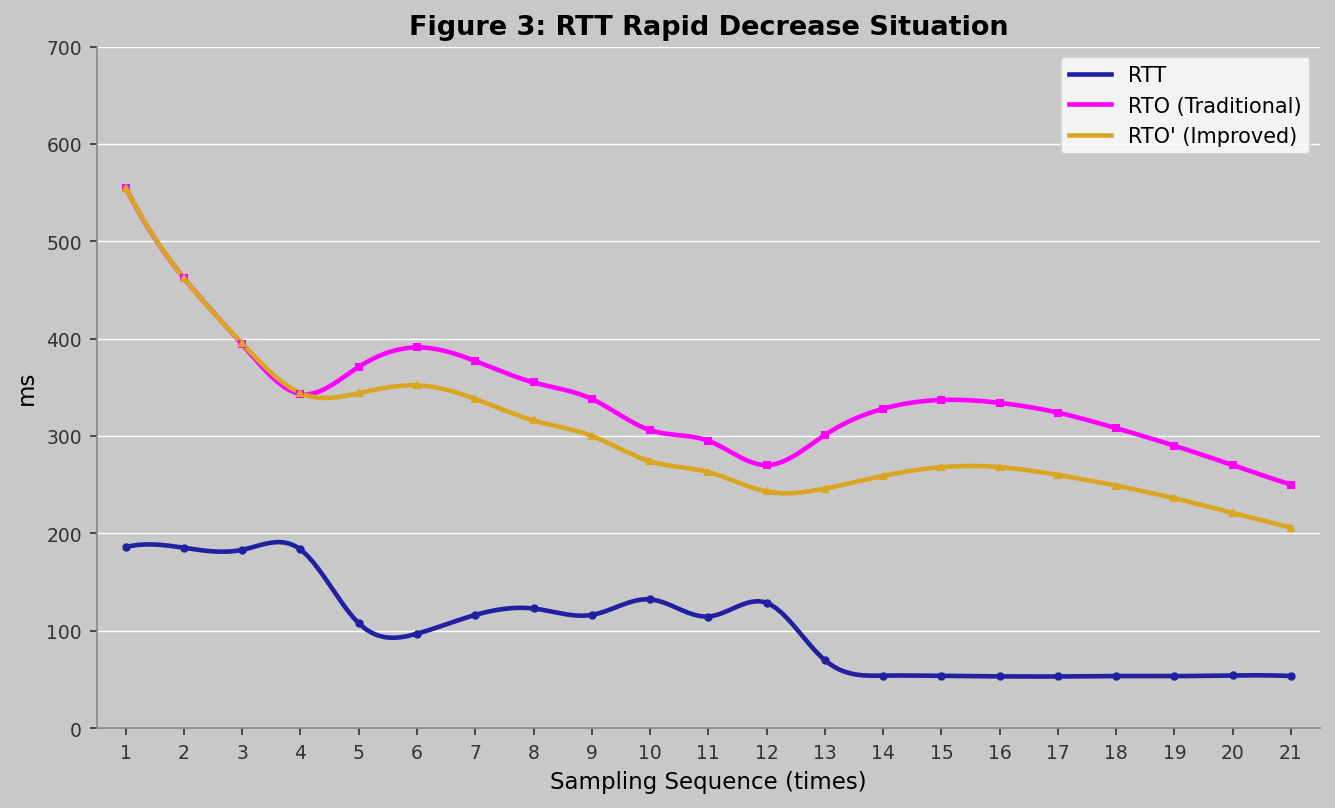
\includegraphics[width=\linewidth]{paper-dual-fig3.png}
    \caption{RTO vs.\ RTT: decreasing-load phase}
  \end{subfigure}
  \caption{Online reproduction of AMEII 2015 paper figures: traditional
           (Jacobson) vs. improved algorithm.}
  \label{fig:paper-online}
\end{figure}

\begin{figure}[H]
  \centering
  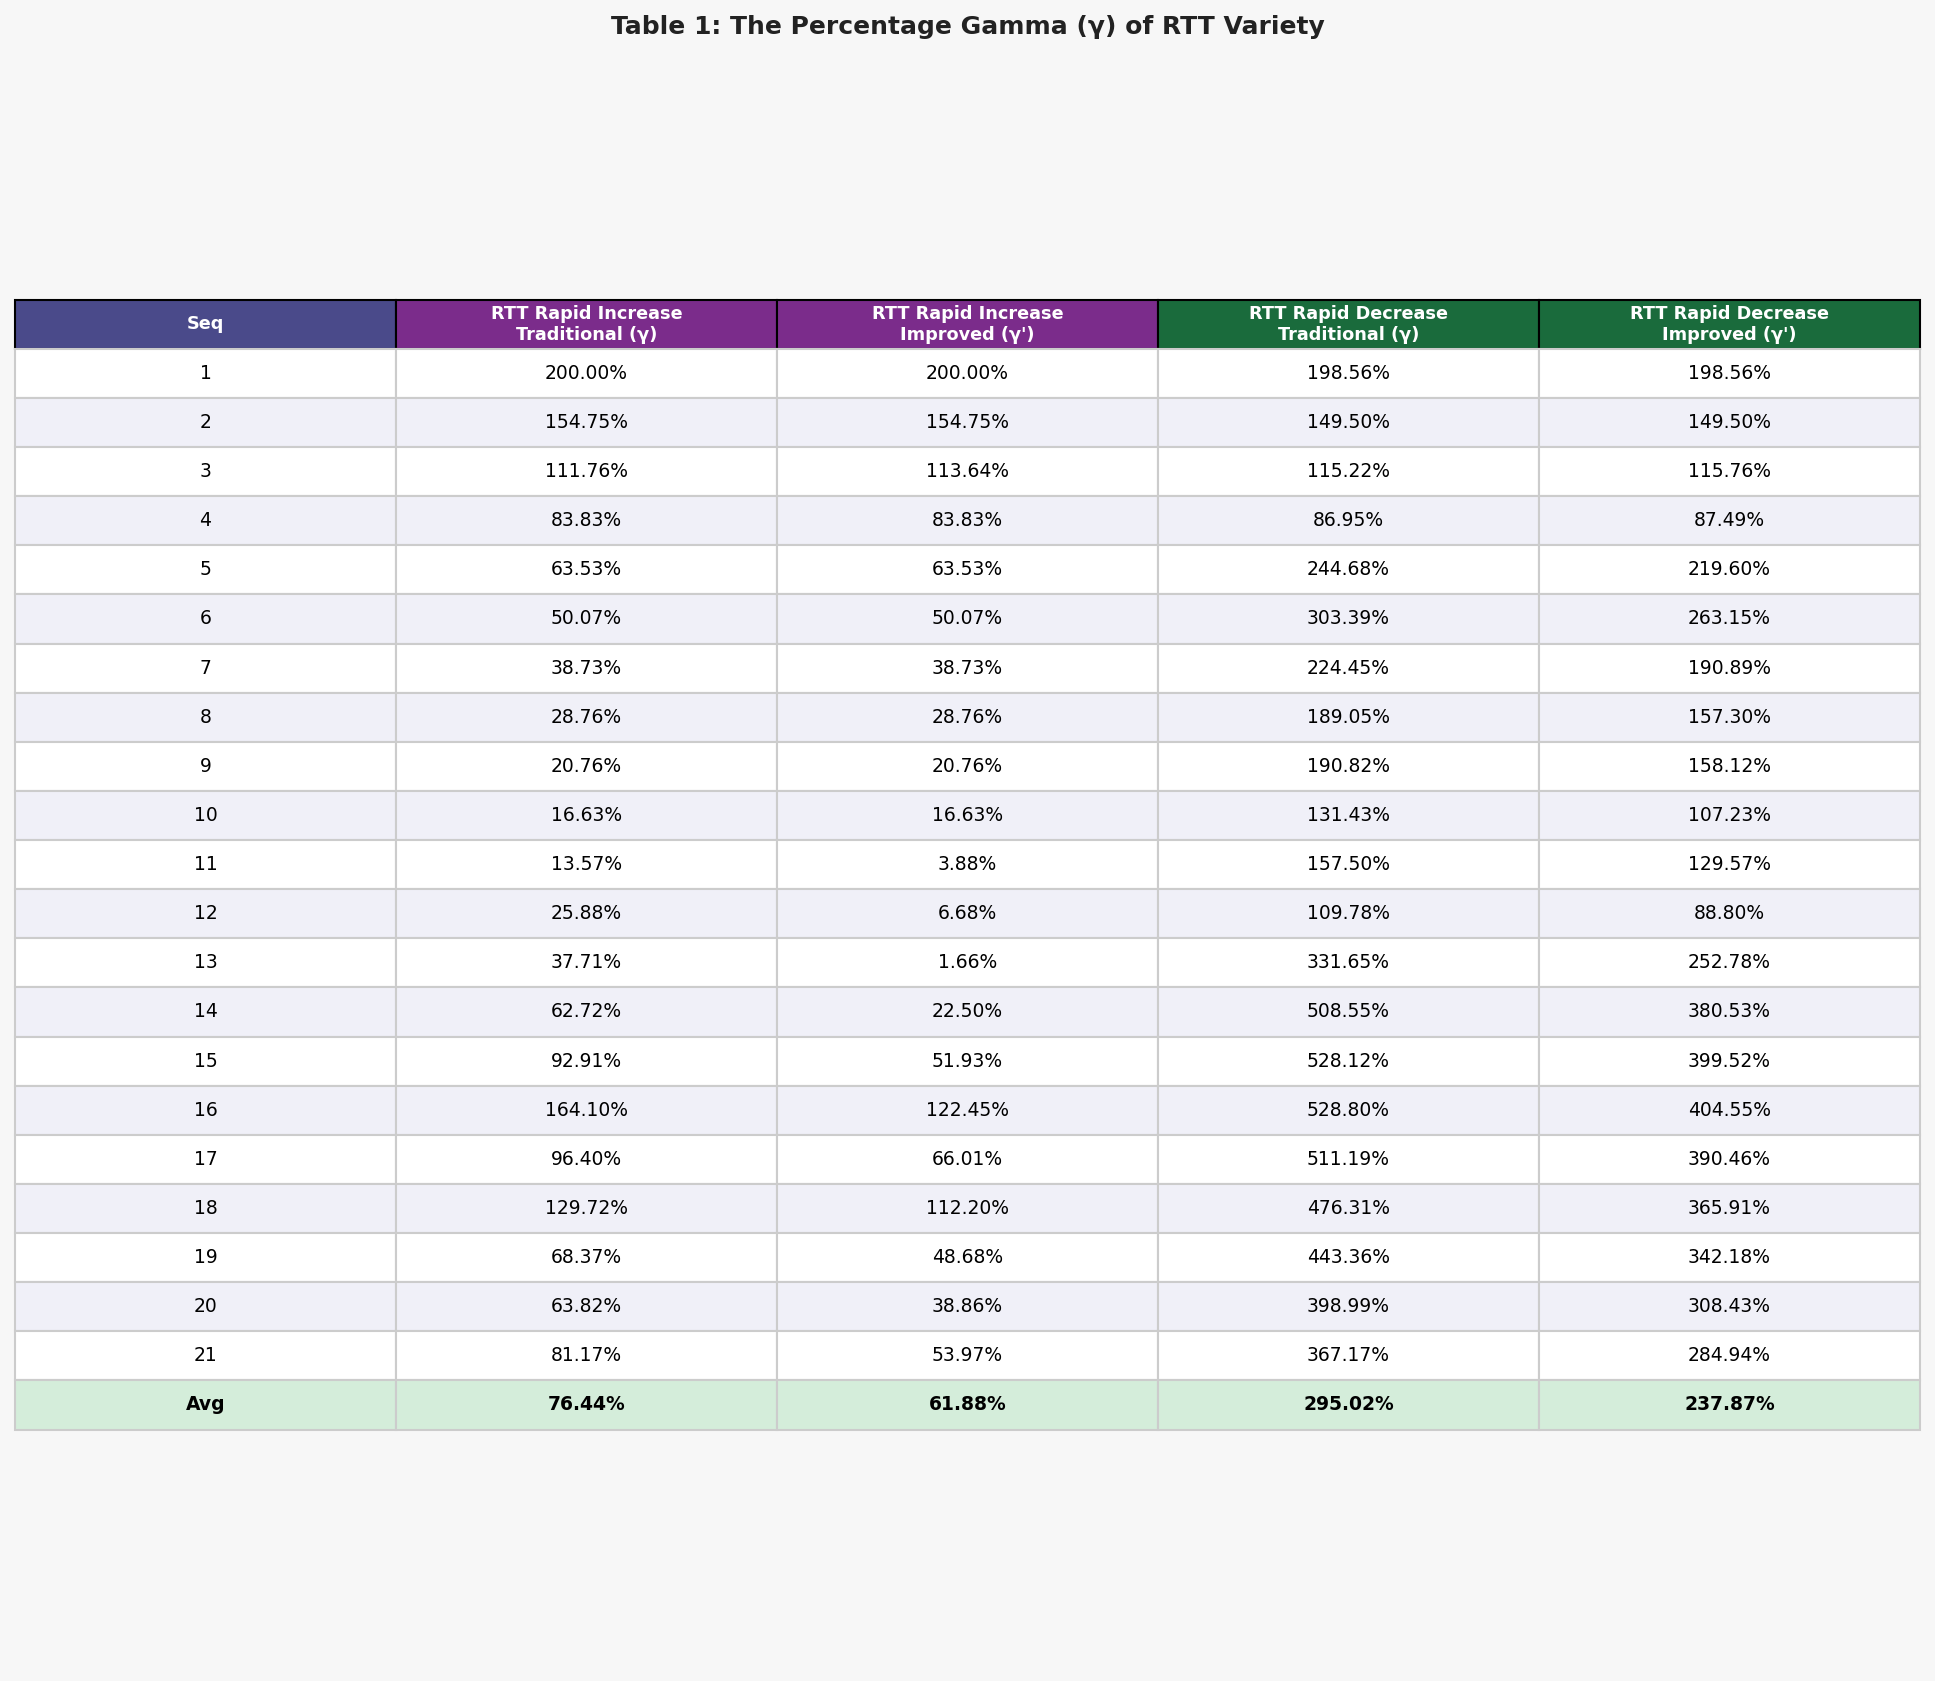
\includegraphics[width=0.65\textwidth]{paper-dual-table1.png}
  \caption{Mean absolute error from paper Table~1 (online reproduction).}
  \label{fig:paper-table1}
\end{figure}

% ═══════════════════════════════════════════════════════════════════════════
\chapter{Proposed Solution and its Logic}
\label{ch:proposed}
% ═══════════════════════════════════════════════════════════════════════════

\section{Limitations of the Paper Algorithm}

While the AMEII 2015 algorithm improves upon Jacobson, it has two weaknesses:
\begin{enumerate}
  \item \textbf{Single-sample trend:}  $k$ is computed from only two
        consecutive RTT samples, making it sensitive to transient noise.
  \item \textbf{No loss awareness:}  Packet loss (a strong indicator of
        congestion) is ignored; the RTO must rely solely on RTT variation.
\end{enumerate}

\section{Proposed Modifications}

The proposed \texttt{RttProposed} algorithm (class \texttt{ns3::RttProposed})
introduces two improvements:

\subsection{Windowed Trend $k_\text{trend}$}

Instead of a single-step ratio, a \emph{window} of $W$ consecutive RTT pairs
is averaged:

\begin{equation}
  k_\text{trend} = \frac{1}{W}\sum_{i=0}^{W-1}
    \frac{|\text{RTT}_{n-i} - \text{RTT}_{n-i-1}|}{\text{RTT}_{n-i-1}}
  \label{eq:ktrend}
\end{equation}

The adaptive weights then follow:
\begin{align}
  \alpha &= \alpha_0 \cdot (1 + k_\text{trend}) \label{eq:alpha-prop} \\
  \beta  &= \beta_0  \cdot (1 - k_\text{trend}) \label{eq:beta-prop}
\end{align}

Averaging over $W$ samples smooths out one-off RTT spikes and yields a more
reliable trend signal.

\subsection{Loss-Aware RTO Scaling}

The final RTO is multiplied by a factor that incorporates the current packet
loss rate, providing a direct congestion signal:

\begin{equation}
  \text{RTO} = \bigl(1 + \gamma \cdot \text{LossRate}\bigr)
               \cdot \bigl(\text{SRTT} + 4 \cdot \text{RTTVAR}\bigr)
  \label{eq:rto-prop}
\end{equation}

\noindent where $\gamma \geq 0$ is a tunable \emph{loss sensitivity factor}.
When $\gamma = 0$ the formula reduces to standard Jacobson/AMEII behaviour.
The best empirically-tuned configuration was $W = 2$, $\gamma = 0.25$.

\subsection{Logical Rationale}

\begin{itemize}
  \item \textbf{Windowed trend:} A window of $W=2$ considers the last two
        RTT differences, reducing the variance in $k_\text{trend}$ and
        preventing the smoothing parameters from swinging wildly.
  \item \textbf{Loss scaling:} Congestion causes both RTT increase
        \emph{and} packet loss.  Scaling RTO by loss rate ensures the timeout
        is generous when the network is genuinely stressed, avoiding the
        spurious-retransmission cascade.
  \item \textbf{Backward compatibility:} Setting $W=1$, $\gamma=0$ exactly
        reproduces the AMEII 2015 behaviour; setting $\alpha_0 = \tfrac{1}{8}$,
        $\beta_0 = \tfrac{1}{4}$ additionally recovers Jacobson.
\end{itemize}

\section{Proposed Algorithm: Comparison Graphs}

\begin{figure}[H]
  \centering
  \begin{subfigure}[t]{0.48\textwidth}
    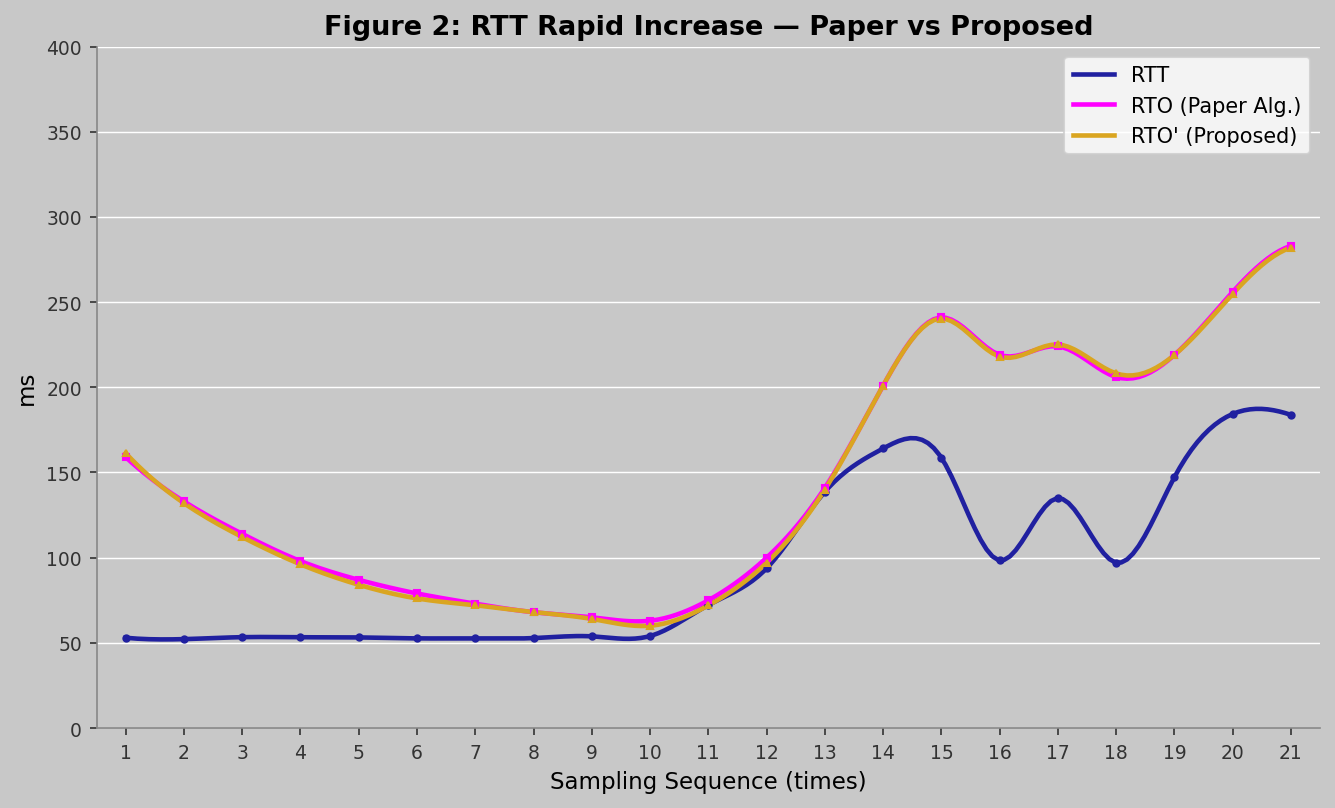
\includegraphics[width=\linewidth]{prop-fig2.png}
    \caption{RTO vs.\ RTT: increasing phase (W=1)}
  \end{subfigure}
  \hfill
  \begin{subfigure}[t]{0.48\textwidth}
    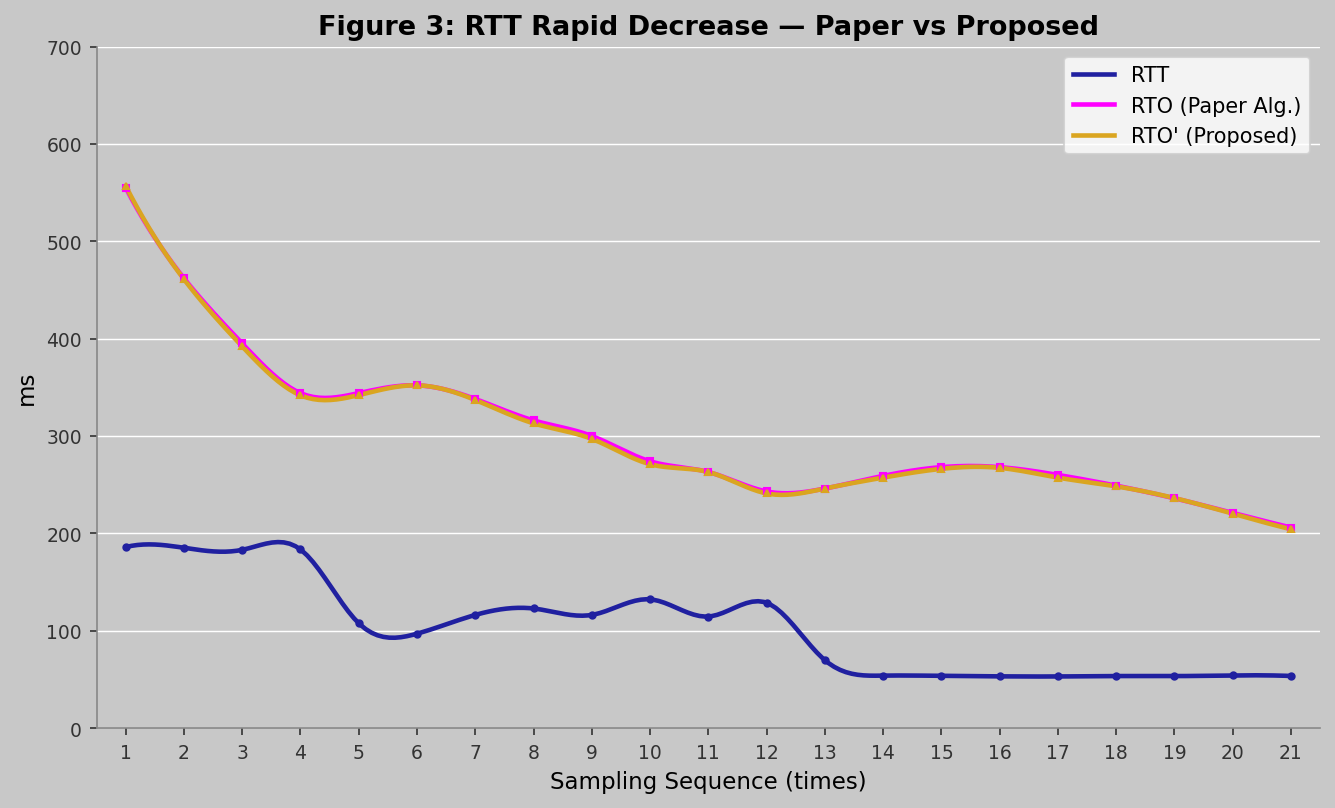
\includegraphics[width=\linewidth]{prop-fig3.png}
    \caption{RTO vs.\ RTT: decreasing phase (W=1)}
  \end{subfigure}
  \caption{Proposed algorithm (W=1) vs.\ paper algorithm.}
  \label{fig:prop-fig23}
\end{figure}

\begin{figure}[H]
  \centering
  \begin{subfigure}[t]{0.48\textwidth}
    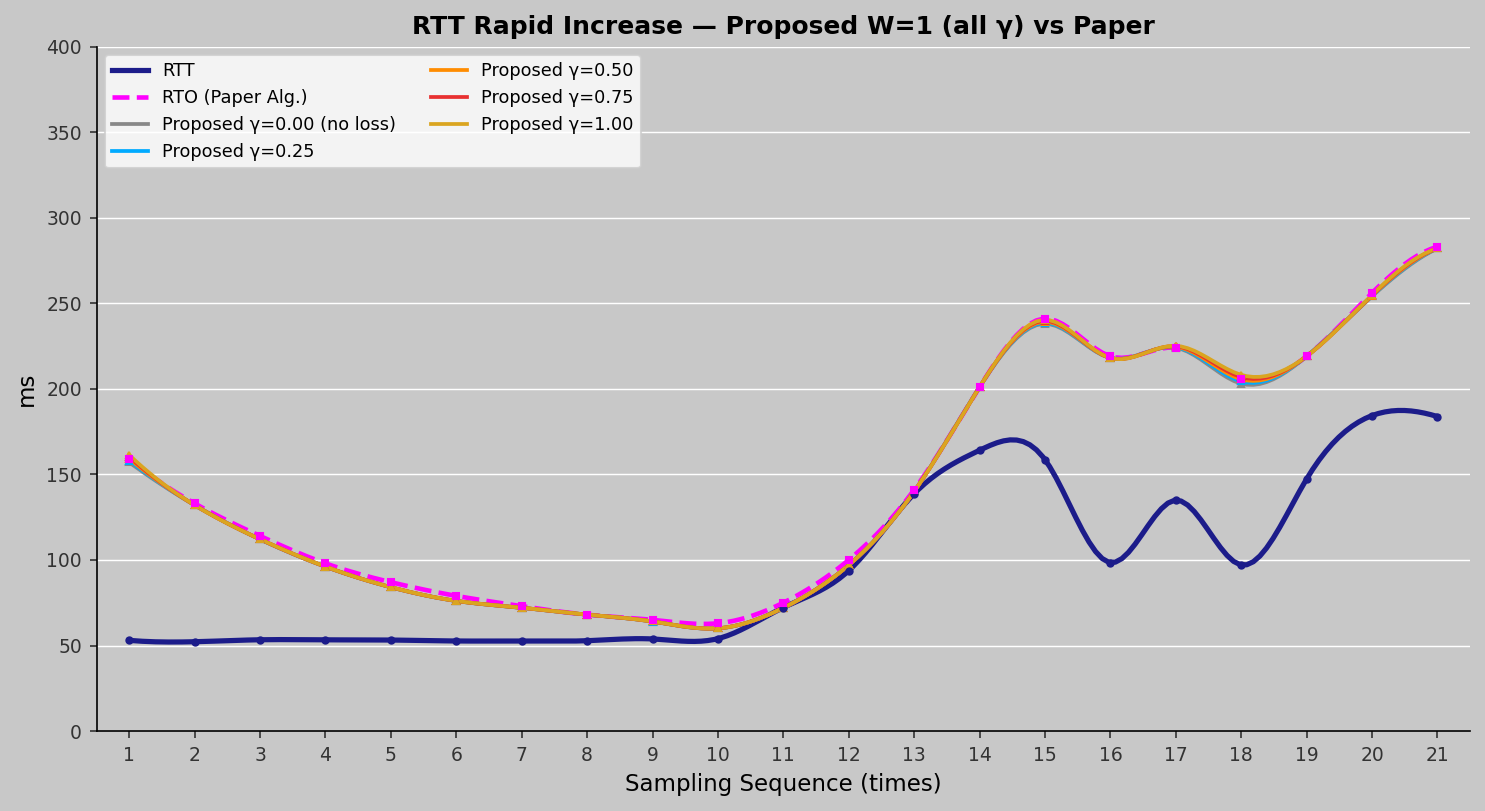
\includegraphics[width=\linewidth]{prop-W1-increase.png}
    \caption{$W=1$, increasing phase}
  \end{subfigure}
  \hfill
  \begin{subfigure}[t]{0.48\textwidth}
    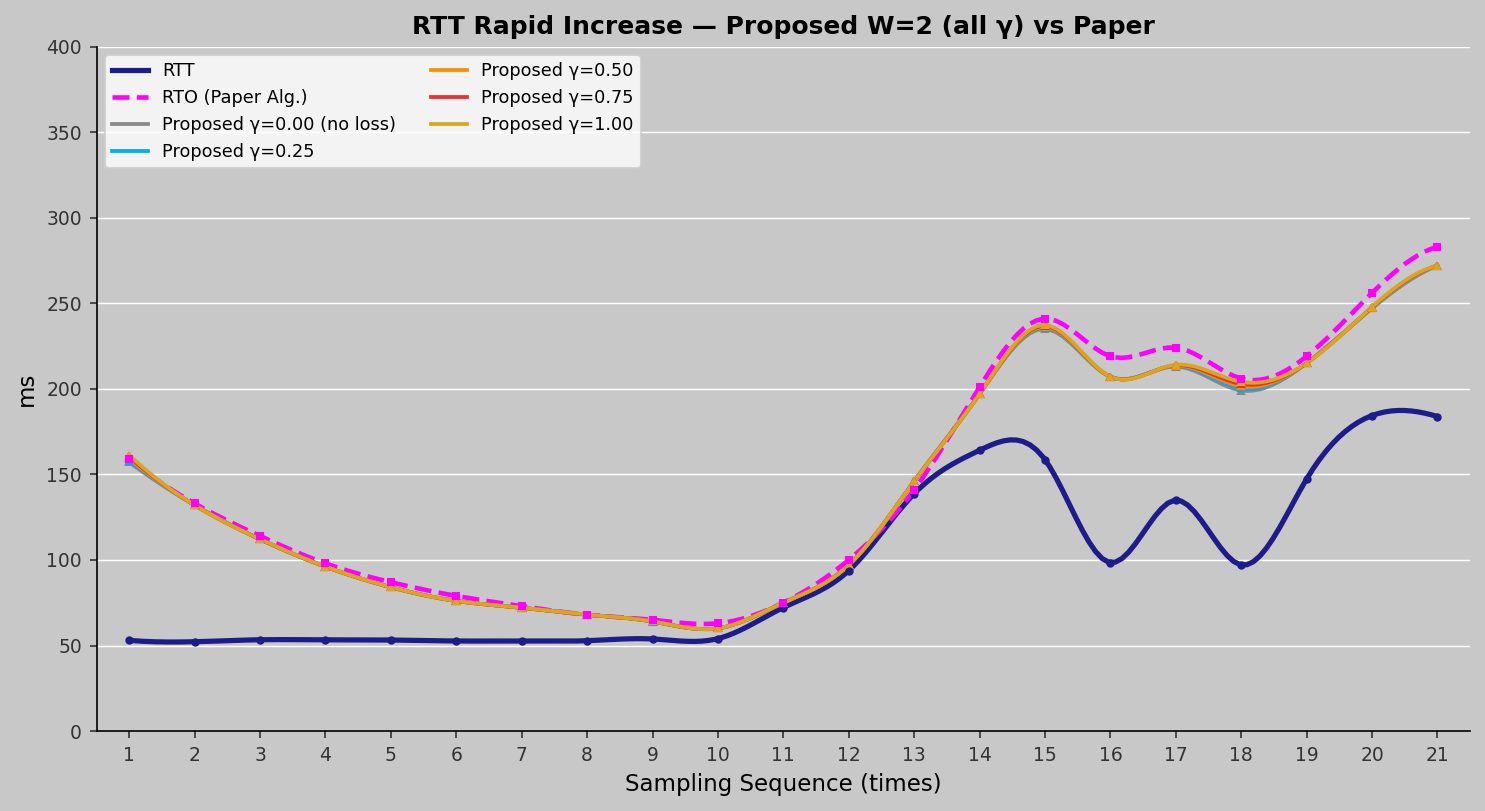
\includegraphics[width=\linewidth]{prop-W2-increase.png}
    \caption{$W=2$, increasing phase}
  \end{subfigure}\\[1em]
  \begin{subfigure}[t]{0.48\textwidth}
    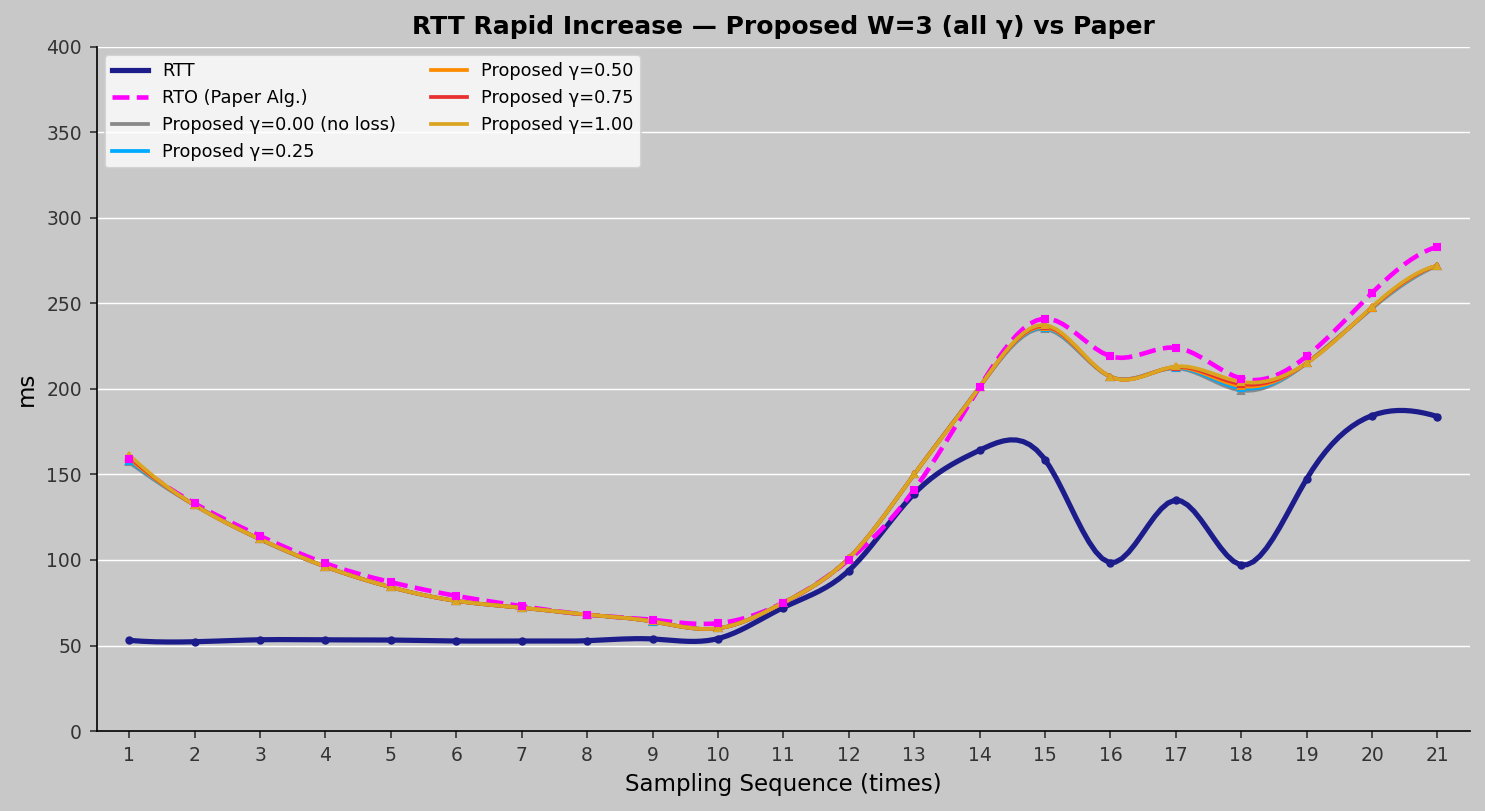
\includegraphics[width=\linewidth]{prop-W3-increase.png}
    \caption{$W=3$, increasing phase}
  \end{subfigure}
  \hfill
  \begin{subfigure}[t]{0.48\textwidth}
    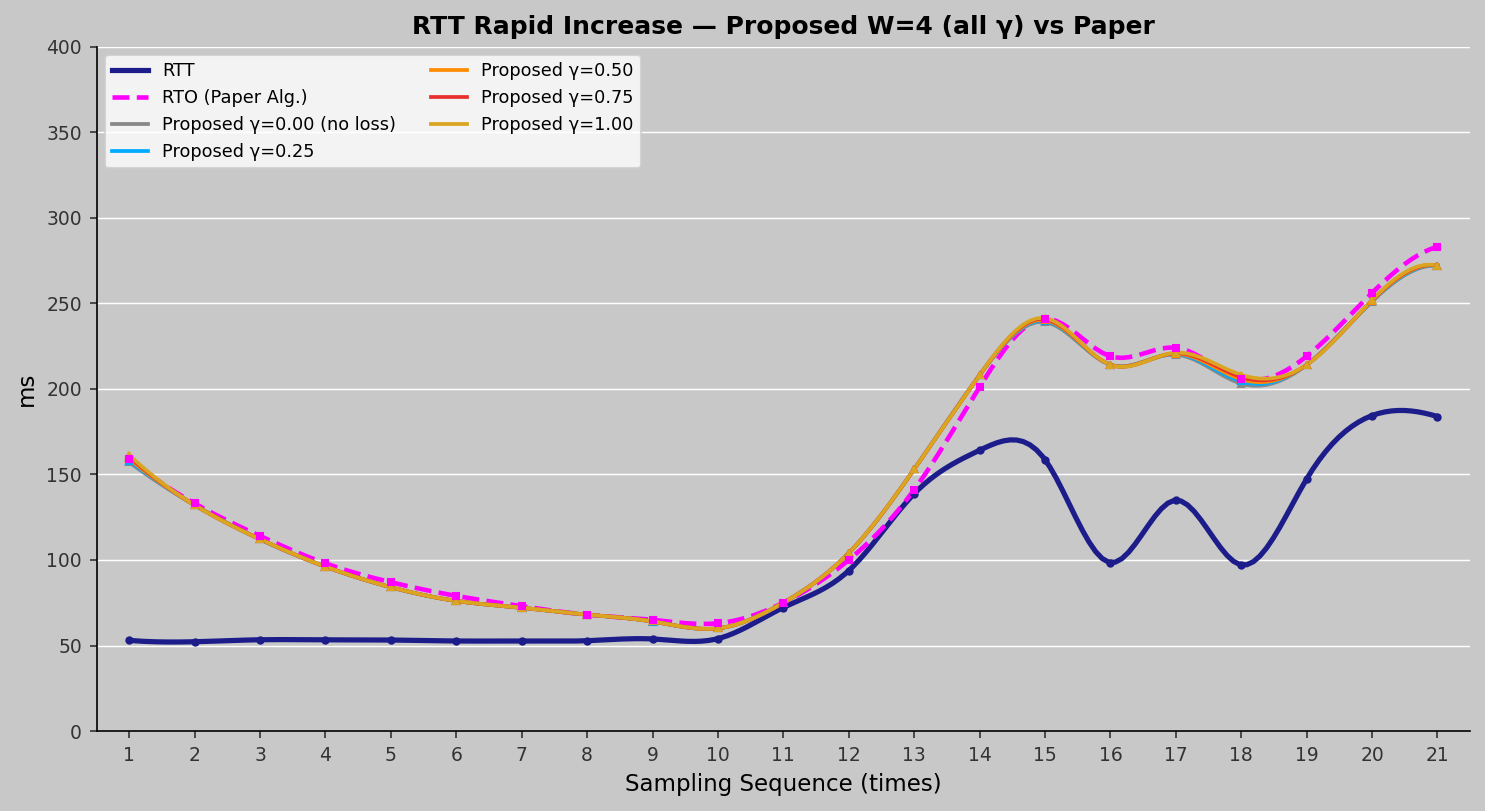
\includegraphics[width=\linewidth]{prop-W4-increase.png}
    \caption{$W=4$, increasing phase}
  \end{subfigure}
  \caption{Effect of window size $W$ on RTO during the increasing-RTT phase.}
  \label{fig:prop-windows-inc}
\end{figure}

\begin{figure}[H]
  \centering
  \begin{subfigure}[t]{0.48\textwidth}
    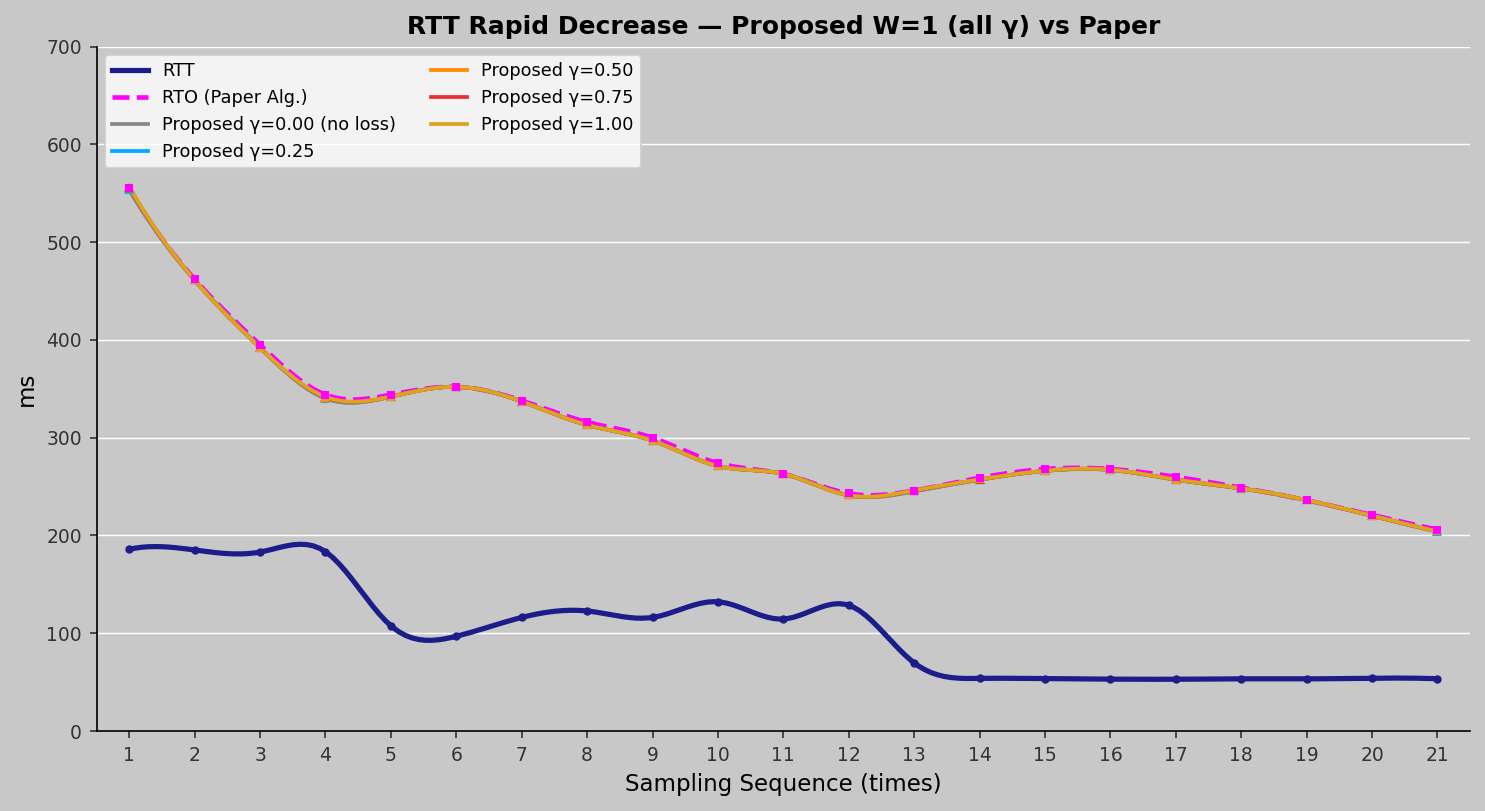
\includegraphics[width=\linewidth]{prop-W1-decrease.png}
    \caption{$W=1$, decreasing phase}
  \end{subfigure}
  \hfill
  \begin{subfigure}[t]{0.48\textwidth}
    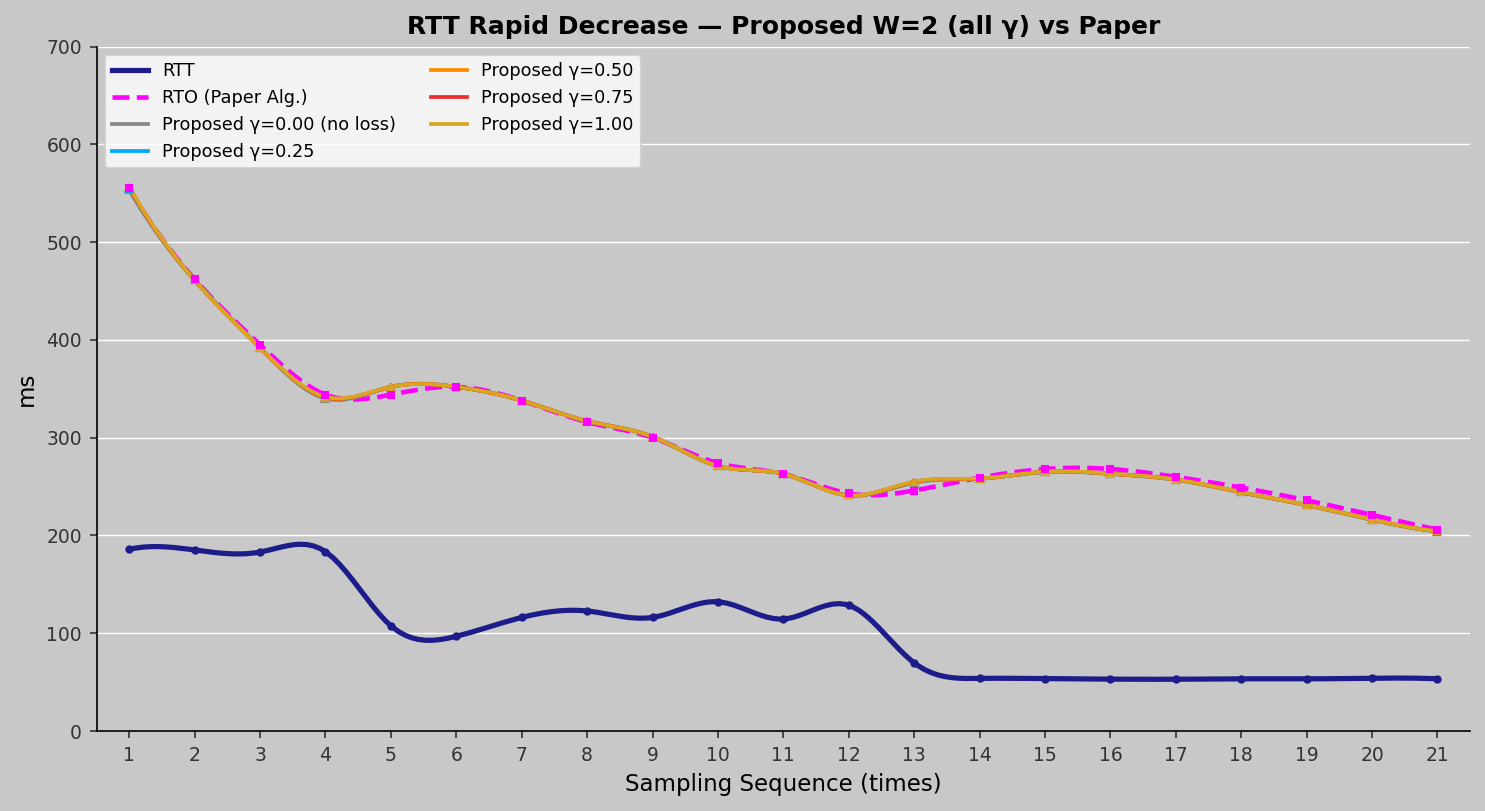
\includegraphics[width=\linewidth]{prop-W2-decrease.png}
    \caption{$W=2$, decreasing phase}
  \end{subfigure}\\[1em]
  \begin{subfigure}[t]{0.48\textwidth}
    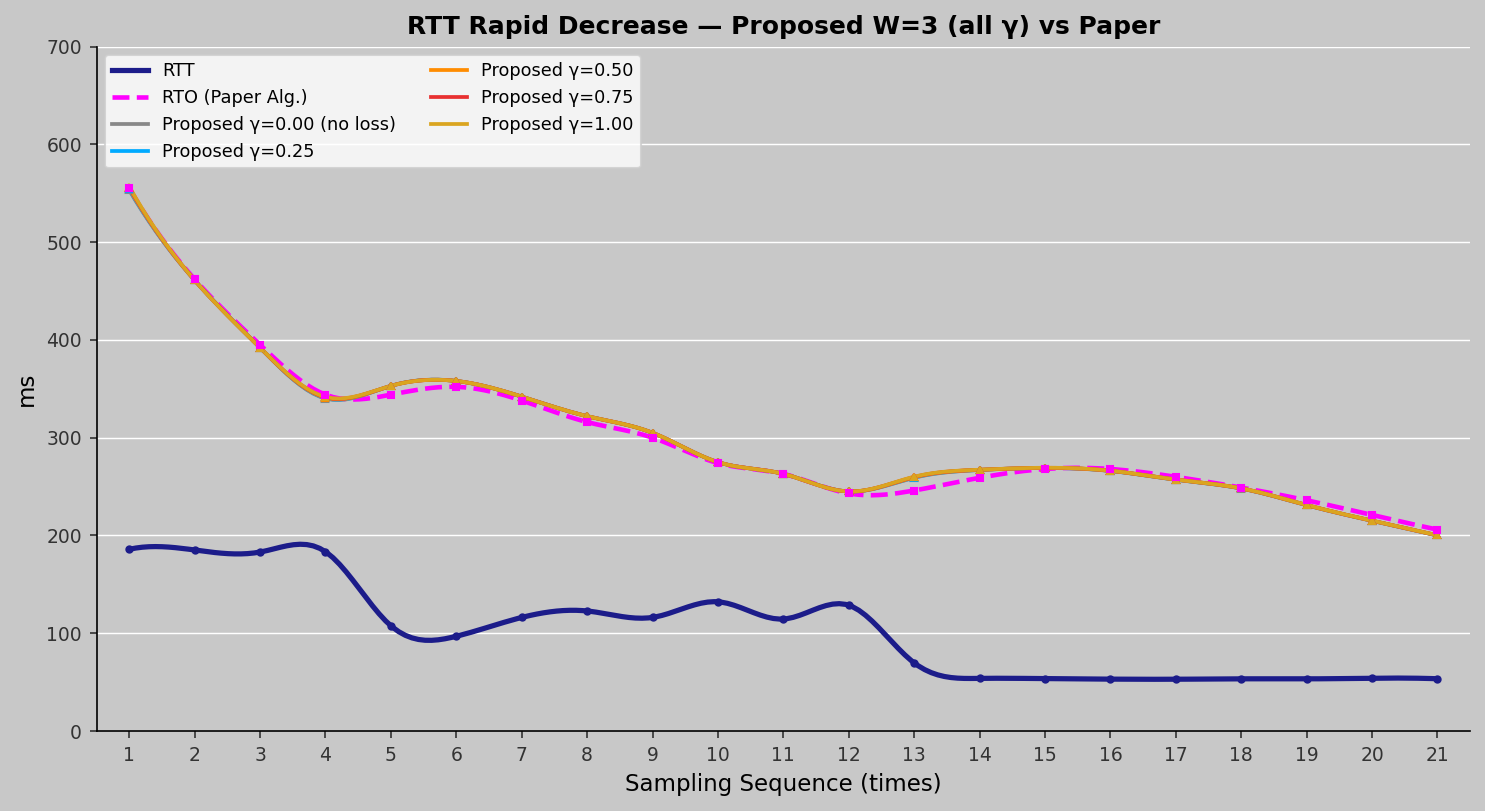
\includegraphics[width=\linewidth]{prop-W3-decrease.png}
    \caption{$W=3$, decreasing phase}
  \end{subfigure}
  \hfill
  \begin{subfigure}[t]{0.48\textwidth}
    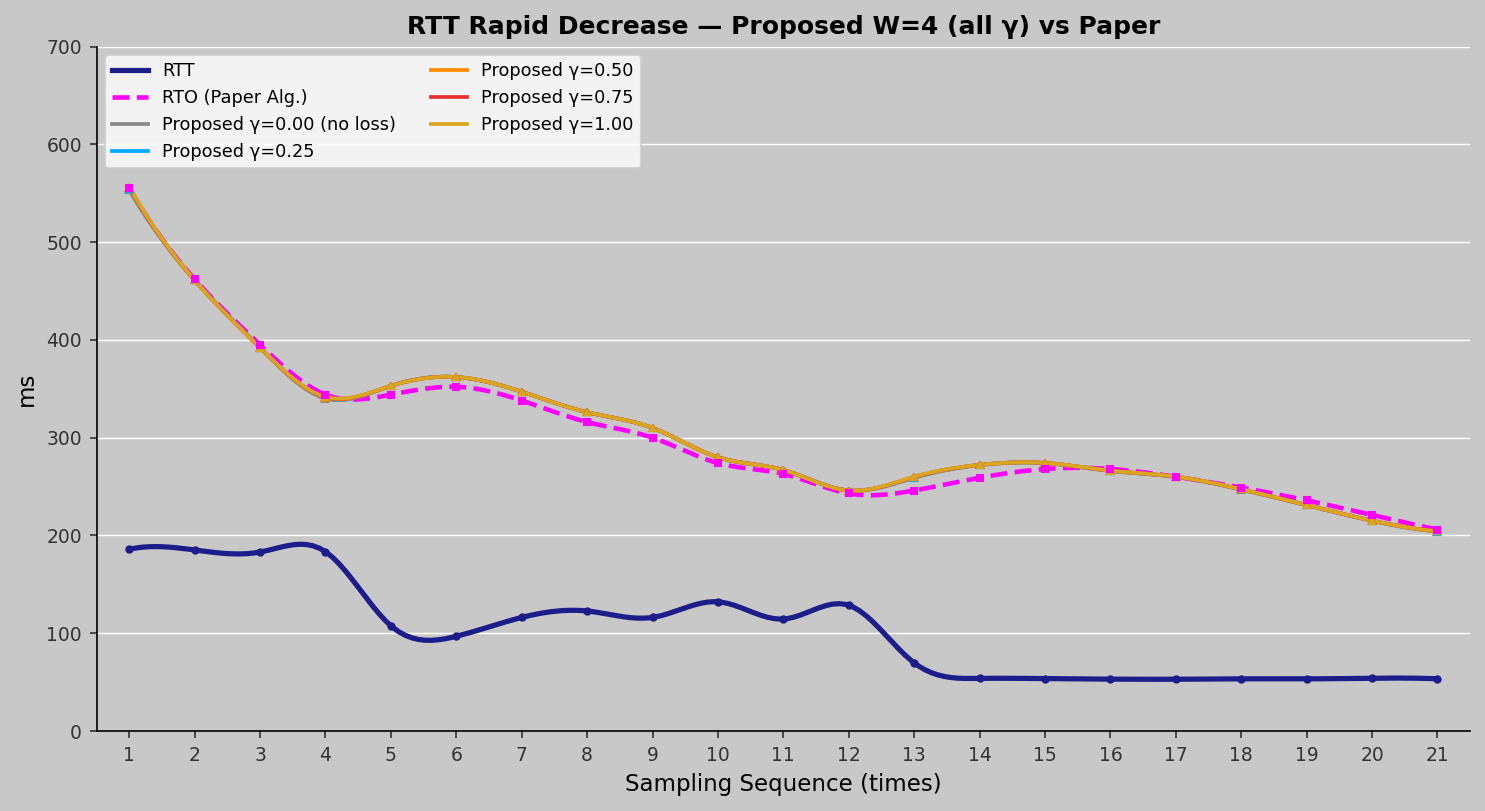
\includegraphics[width=\linewidth]{prop-W4-decrease.png}
    \caption{$W=4$, decreasing phase}
  \end{subfigure}
  \caption{Effect of window size $W$ on RTO during the decreasing-RTT phase.}
  \label{fig:prop-windows-dec}
\end{figure}

\begin{figure}[H]
  \centering
  \begin{subfigure}[t]{0.48\textwidth}
    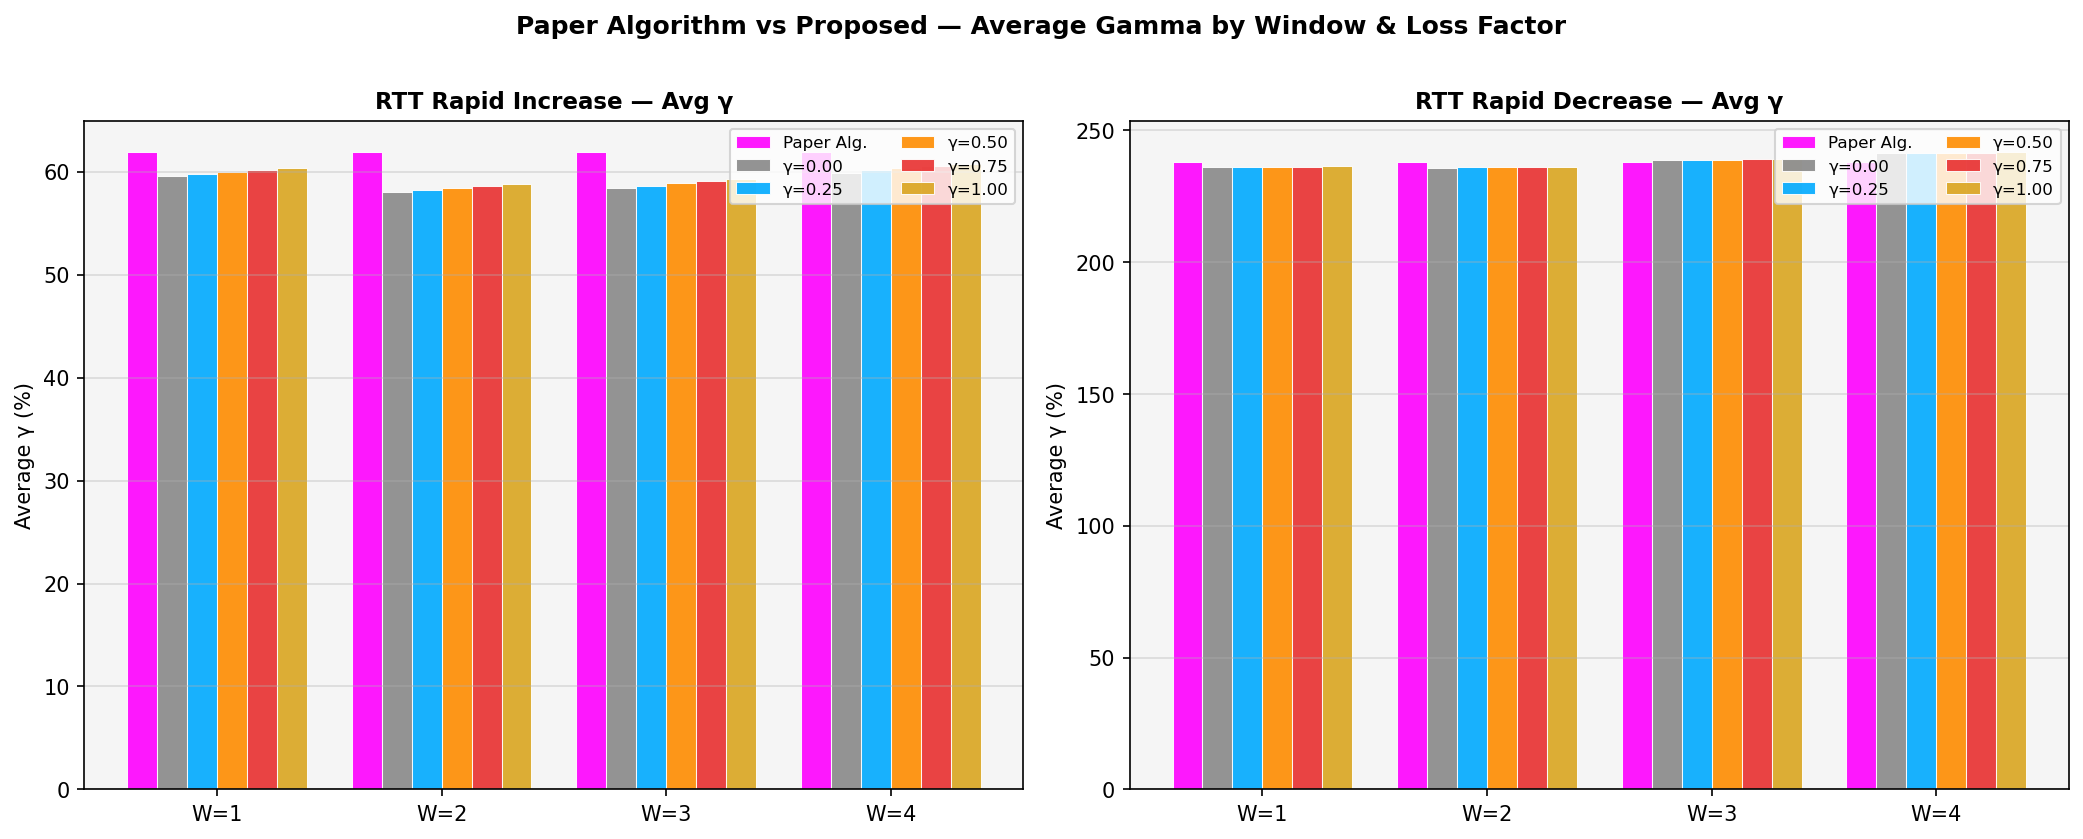
\includegraphics[width=\linewidth]{prop-bar-summary.png}
    \caption{Bar-chart: mean absolute deviation}
  \end{subfigure}
  \hfill
  \begin{subfigure}[t]{0.48\textwidth}
    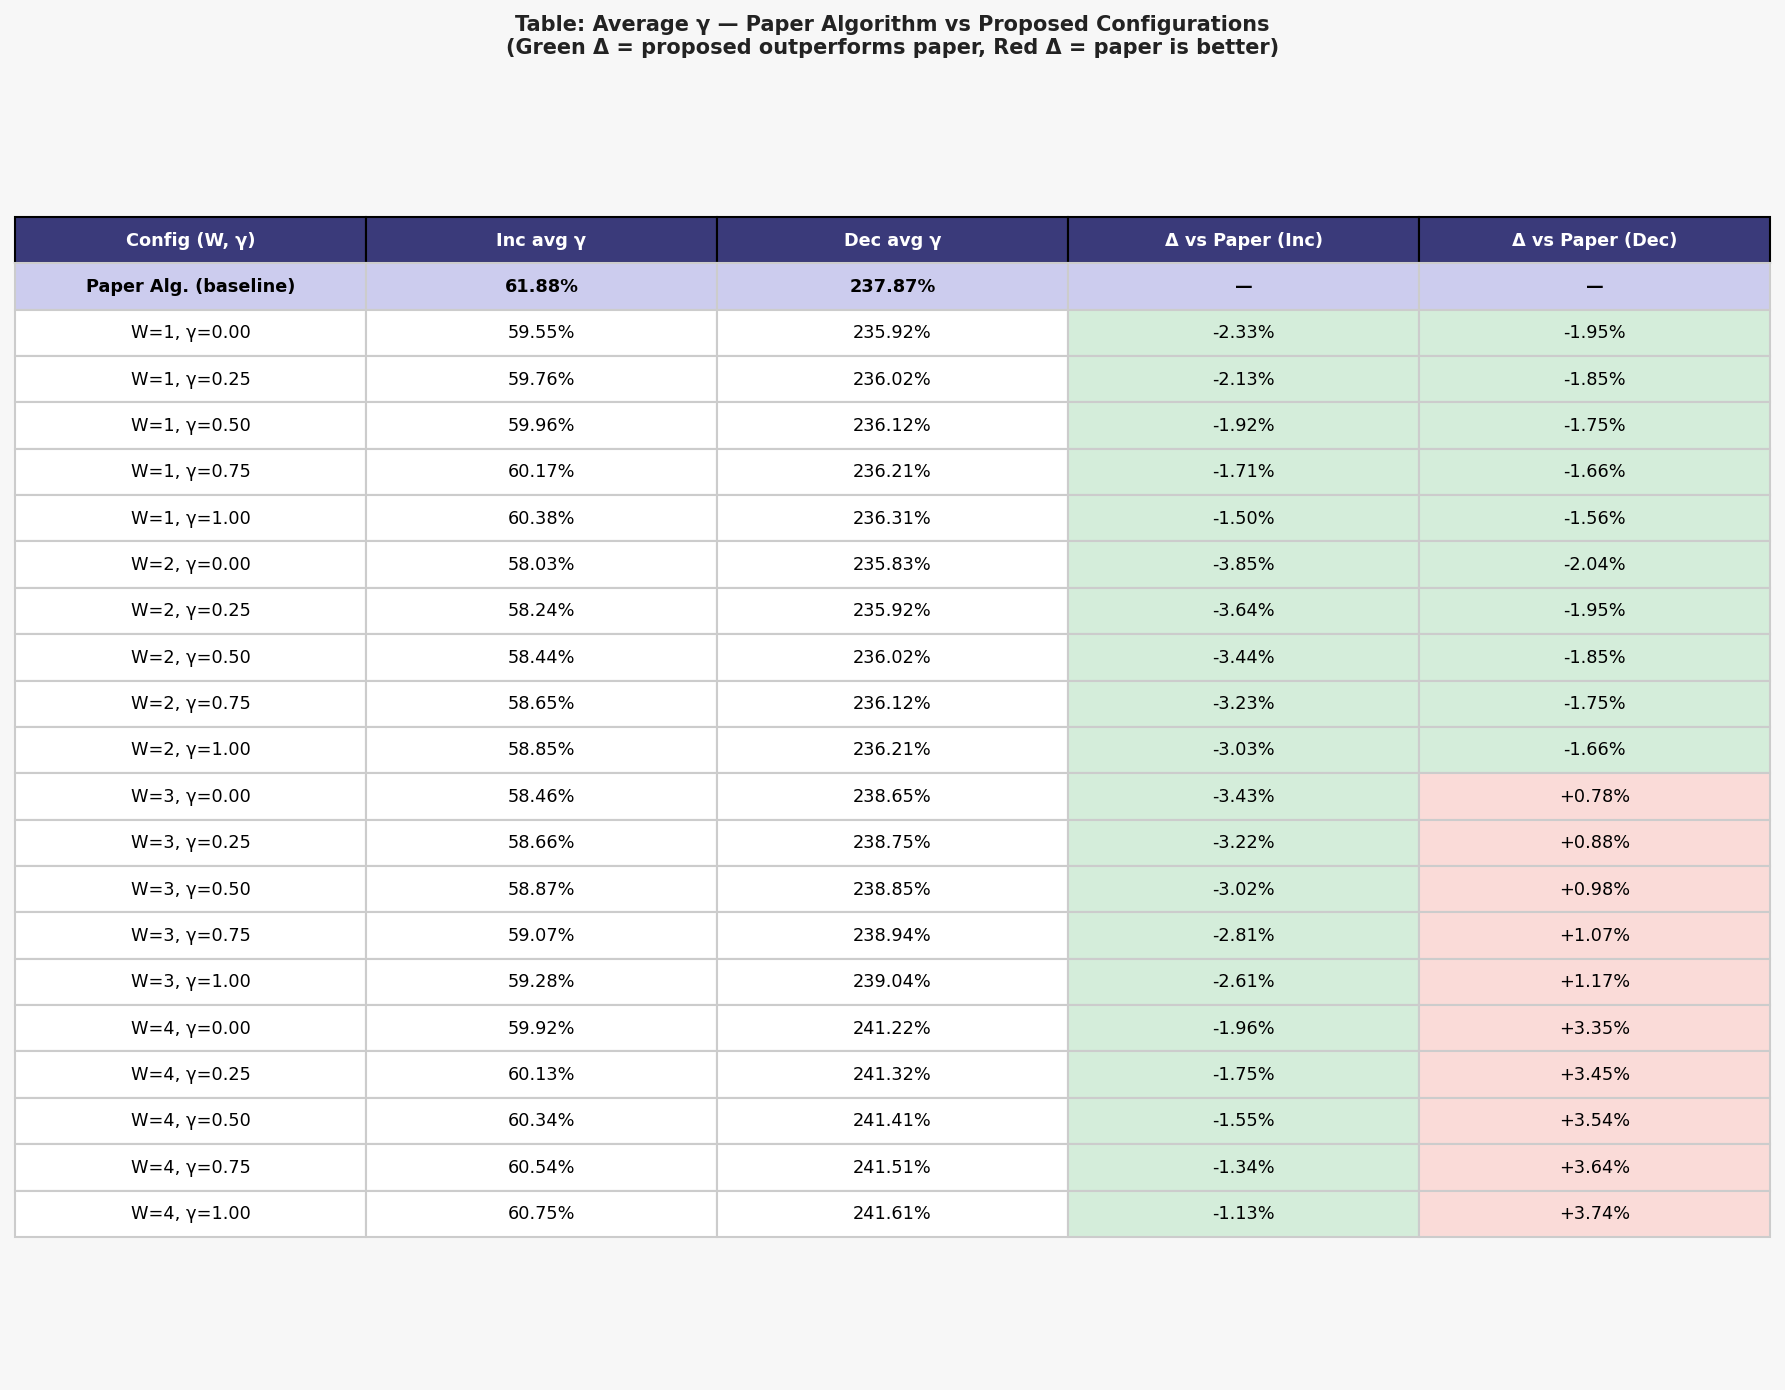
\includegraphics[width=\linewidth]{prop-summary-table.png}
    \caption{Summary table by window size}
  \end{subfigure}
  \caption{Proposed algorithm summary across window sizes $W \in \{1,2,3,4\}$.}
  \label{fig:prop-summary}
\end{figure}

% ═══════════════════════════════════════════════════════════════════════════
\chapter{Classes Implemented in the Simulator}
\label{ch:classes}
% ═══════════════════════════════════════════════════════════════════════════

Three main C++ classes were written or integrated into ns-3.45:

\section{\texttt{ns3::RttImprovedEstimator}
         (\texttt{contrib/improved-rto2/model/})}

This class implements the AMEII 2015 paper algorithm.  It inherits from
\texttt{ns3::RttMeanDeviation} (the standard Jacobson estimator) and overrides
\texttt{Measurement(Time t)} to apply Equations~\ref{eq:k}--\ref{eq:beta-paper}.

\begin{lstlisting}[style=cppstyle, caption={Key
    attributes of \texttt{RttImprovedEstimator}}]
static TypeId tid = TypeId("ns3::RttImprovedEstimator")
    .SetParent<RttMeanDeviation>()
    .AddAttribute("Alpha0",
                  "Base gain for SRTT (default 1/8)",
                  DoubleValue(0.125), ...)
    .AddAttribute("Beta0",
                  "Base gain for RTTVAR (default 1/4)",
                  DoubleValue(0.25), ...);
\end{lstlisting}

\textbf{Key internal members:}
\begin{description}[leftmargin=3cm, style=nextline]
  \item[\texttt{m\_alpha0}]  Base $\alpha_0$ (default $0.125$)
  \item[\texttt{m\_beta0}]   Base $\beta_0$ (default $0.25$)
  \item[\texttt{m\_prevRtt}] Previous RTT sample for $k$ computation
  \item[\texttt{m\_hasPrev}] Boolean guard (skip $k$ on first sample)
\end{description}

\textbf{Algorithm in \texttt{Measurement()}:}
\begin{enumerate}
  \item Compute $k = |t - \texttt{m\_prevRtt}| / \texttt{m\_prevRtt}$, capped at~1.
  \item Set $\alpha = \alpha_0(1+k)$, $\beta = \beta_0(1-k)$.
  \item Update SRTT via EWMA with $\alpha$.
  \item Update RTTVAR via EWMA with $\beta$.
  \item Store $t$ as \texttt{m\_prevRtt}.
\end{enumerate}

\section{\texttt{ns3::RttProposed}
         (\texttt{src/improved-rto/model/})}

This class implements the proposed loss-aware, windowed-trend algorithm.  It
inherits directly from \texttt{ns3::RttEstimator} (not from the paper class,
to keep a clean derivation) and overrides \texttt{Measurement(Time t)}.

\begin{lstlisting}[style=cppstyle, caption={Key
    attributes of \texttt{RttProposed}}]
static TypeId tid = TypeId("ns3::RttProposed")
    .SetParent<RttEstimator>()
    .AddAttribute("Alpha0",  ..., DoubleValue(0.125), ...)
    .AddAttribute("Beta0",   ..., DoubleValue(0.25),  ...)
    .AddAttribute("WindowSize",
                  "W -- trend window (1..100)",
                  UintegerValue(1), ...)
    .AddAttribute("Gamma",
                  "Loss sensitivity factor",
                  DoubleValue(1.0), ...);
\end{lstlisting}

\textbf{Key internal members:}
\begin{description}[leftmargin=3.5cm, style=nextline]
  \item[\texttt{m\_alpha0, m\_beta0}] Baseline smoothing factors
  \item[\texttt{m\_windowSize}]       $W$ -- trend window (default~1)
  \item[\texttt{m\_gamma}]            Loss sensitivity $\gamma$ (default~1.0)
  \item[\texttt{m\_lossRate}]         Current packet loss rate (0--1), set externally
  \item[\texttt{m\_rttHistory}]       \texttt{std::deque<Time>} holding last $W+1$ RTT samples
  \item[\texttt{m\_firstSample}]      Boolean guard for first measurement
\end{description}

\textbf{Public API beyond standard RTT estimator:}
\begin{itemize}
  \item \texttt{SetLossRate(double)} / \texttt{GetLossRate()} -- inject the
        current loss rate from the transport layer.
  \item \texttt{GetGamma()} -- read the configured $\gamma$.
  \item \texttt{GetWindowSize()} -- read $W$.
\end{itemize}

\section{Simulation Scripts}

\subsection{\texttt{scratch/online/paper-rto-dual.cc}}

Reproduces the paper's Figures~2 and~3 through an \emph{online} (in-simulator)
RTO computation.  A 9-flow dumbbell is run for 180\,s.  Flows are added and
removed every 10\,s to generate a natural load ramp.  At 21 checkpoints per
phase the aggregated RTT is fed into both estimators.

\subsection{\texttt{scratch/proposed/paper-rto-proposed.cc}}

Extends the online experiment to sweep window sizes $W \in \{1,2,3,4\}$ and
compares the proposed estimator against the paper algorithm.

\subsection{\texttt{scratch/submission\_checklist/wired/wired-sim.cc}}

Full wired simulation: dumbbell topology, TCP NewReno, FlowMonitor.
Runs both algorithms across a grid of (nodes, flows, pps) values and
appends measured throughput, delay, PDR, and drop ratio to a CSV file.

\subsection{\texttt{scratch/submission\_checklist/wireless/wireless-sim.cc}}

Full wireless simulation: 802.11g AdHoc static grid, AODV, UDP OnOff,
BasicEnergySource, FlowMonitor.  Sweeps (nodes, flows, pps, coverage).
Appends throughput, delay, PDR, drop ratio, and energy to CSV.

% ═══════════════════════════════════════════════════════════════════════════
\chapter{Network Topologies Under Simulation}
\label{ch:topology}
% ═══════════════════════════════════════════════════════════════════════════

\section{Wired Dumbbell Topology}

\begin{figure}[H]
  \centering
  \setlength{\unitlength}{1pt}
  \begin{picture}(340,90)
    % Left senders
    \put(0,60){\circle*{5}}  \put(3,62){\small $S_0$}
    \put(0,40){\circle*{5}}  \put(3,42){\small $S_1$}
    \put(0,20){\circle*{5}}  \put(3,22){\small $\vdots$}
    % R1
    \put(100,40){\circle{12}} \put(96,38){\small $R_1$}
    % Bottleneck
    \put(106,40){\line(1,0){128}}
    % R2
    \put(240,40){\circle{12}} \put(236,38){\small $R_2$}
    % Right receivers
    \put(340,60){\circle*{5}} \put(318,62){\small $D_0$}
    \put(340,40){\circle*{5}} \put(318,42){\small $D_1$}
    \put(340,20){\circle*{5}} \put(318,22){\small $\vdots$}
    % Access links
    \put(0,60){\line(5,-1){93}}
    \put(0,40){\line(1,0){94}}
    \put(0,20){\line(5,1){93}}
    \put(246,40){\line(5,-1){88}}
    \put(246,40){\line(1,0){88}}
    \put(246,40){\line(5,1){88}}
    % Labels
    \put(35,55){\tiny 100 Mbps / 1 ms}
    \put(135,45){\tiny 100 Mbps / 10 ms}
    \put(270,55){\tiny 100 Mbps / 1 ms}
  \end{picture}
  \caption{Wired dumbbell topology. $N/2$ senders on the left,
           $N/2$ receivers on the right; $R_1$--$R_2$ is the shared
           bottleneck link.}
  \label{fig:dumbbell}
\end{figure}

\begin{table}[H]
  \centering
  \caption{Wired topology link parameters}
  \label{tab:wired-links}
  \begin{tabular}{llll}
    \toprule
    \textbf{Link type} & \textbf{Data Rate} & \textbf{Delay} & \textbf{Queue} \\
    \midrule
    Access (sender-to-$R_1$)    & 100 Mbps & 1 ms  & DropTail (default) \\
    Bottleneck ($R_1$--$R_2$)   & 100 Mbps & 10 ms & DropTail 100 packets \\
    Access ($R_2$-to-receiver)  & 100 Mbps & 1 ms  & DropTail (default) \\
    \bottomrule
  \end{tabular}
\end{table}

\textbf{Transport:} TCP NewReno with 512-byte segments and 1\,MB socket buffers.
Each of the $F$ TCP flows is created from a unique sender to its paired receiver.
Flows start at $t=1$\,s and stop at $t=\text{simTime}-1$\,s.

\section{Wireless 802.11g Ad-Hoc Static Topology}

\begin{table}[H]
  \centering
  \caption{Wireless topology parameters}
  \label{tab:wireless-params}
  \begin{tabular}{ll}
    \toprule
    \textbf{Parameter}      & \textbf{Value} \\
    \midrule
    MAC / PHY standard      & 802.11g (YansWifi, AdHoc mode) \\
    PHY data rate           & 54 Mbps (OfdmRate54Mbps) \\
    Tx range                & $\approx 250$\,m \\
    Node placement          & Regular grid, spacing = coverage\,/\,$\sqrt{N}$ \\
    Mobility model          & ConstantPositionMobilityModel (static) \\
    Routing protocol        & AODV \\
    Application             & UDP OnOff (no TCP RTO effect -- rate measured by FlowMonitor) \\
    Energy model            & BasicEnergySource + WifiRadioEnergyModel \\
    Initial energy          & 100\,J per node \\
    \bottomrule
  \end{tabular}
\end{table}

\noindent Nodes are laid out on a square grid.  The coverage side length is
one of $\{250, 500, 750, 1000, 1250\}$\,m, corresponding to $1\times$ through
$5\times$ the nominal Wi-Fi transmission range of 250\,m.  AODV discovers
routes before flows start (flows begin at $t=3$\,s).

% ═══════════════════════════════════════════════════════════════════════════
\chapter{Parameters Under Variation}
\label{ch:params}
% ═══════════════════════════════════════════════════════════════════════════

All experiments vary one parameter at a time while holding the others at their
default values (``one-factor-at-a-time'' design).

\begin{table}[H]
  \centering
  \caption{Wired simulation parameter sweep}
  \label{tab:wired-sweep}
  \begin{tabular}{lllll}
    \toprule
    \textbf{Parameter} & \textbf{Values Swept} & \textbf{Default} & \textbf{Unit} \\
    \midrule
    Number of nodes (\texttt{--nodes}) & 20, 40, 60, 80, 100 & 60 & --- \\
    Number of TCP flows (\texttt{--flows}) & 10, 20, 30, 40, 50 & 30 & --- \\
    Packets per second (\texttt{--pps}) & 100, 200, 300, 400, 500 & 300 & pkt/s \\
    Algorithm (\texttt{--algo}) & paper, proposed & paper & --- \\
    \bottomrule
  \end{tabular}
\end{table}

\begin{table}[H]
  \centering
  \caption{Wireless simulation parameter sweep}
  \label{tab:wireless-sweep}
  \begin{tabular}{lllll}
    \toprule
    \textbf{Parameter} & \textbf{Values Swept} & \textbf{Default} & \textbf{Unit} \\
    \midrule
    Number of nodes (\texttt{--nodes})   & 20, 40, 60, 80, 100 & 60 & --- \\
    Number of flows (\texttt{--flows})   & 10, 20, 30, 40, 50  & 30 & --- \\
    Packets per second (\texttt{--pps}) & 100, 200, 300, 400, 500 & 300 & pkt/s \\
    Coverage side (\texttt{--coverage}) & 250, 500, 750, 1000, 1250 & 750 & metres \\
    Algorithm (\texttt{--algo}) & paper, proposed & paper & --- \\
    \bottomrule
  \end{tabular}
\end{table}

\noindent \textbf{Collected metrics (both topologies):}
throughput (Mbps), end-to-end delay (ms), Packet Delivery Ratio (PDR),
packet drop ratio.  The wireless scenario additionally records total energy
consumed (J) across all nodes.

% ═══════════════════════════════════════════════════════════════════════════
\chapter{Modifications Made in the Simulator}
\label{ch:mods}
% ═══════════════════════════════════════════════════════════════════════════

\section{New RTO Estimator Module: \texttt{src/improved-rto/}}

A standalone ns-3 module was created at \texttt{src/improved-rto/} containing:

\begin{itemize}
  \item \texttt{model/rtt-proposed.h} / \texttt{rtt-proposed.cc} ---
        the \texttt{RttProposed} class (loss-aware, windowed-trend estimator).
  \item \texttt{model/rtt-improved-paper.h} / \texttt{rtt-improved-paper.cc} ---
        an internal copy of the paper class for cross-referencing.
  \item \texttt{CMakeLists.txt} --- registers the module with the ns-3 build
        system so it can be used from any scratch script.
\end{itemize}

The module is registered via CMake's \texttt{build\_lib} macro, which
automatically generates \texttt{ns3/rtt-proposed.h} in the include path.

\section{New Contrib Module: \texttt{contrib/improved-rto2/}}

The AMEII 2015 paper implementation is separately packaged as an ns-3
contribution module so that it can be cleanly swapped in via:

\begin{lstlisting}[style=cppstyle]
Config::SetDefault("ns3::TcpL4Protocol::RttEstimatorType",
                   TypeIdValue(RttImprovedEstimator::GetTypeId()));
\end{lstlisting}

\noindent Both modules are installed and built with the standard CMake
workflow (\texttt{./ns3 configure \&\& ./ns3 build}).

\section{Algorithm Selection in Simulation Scripts}

The \texttt{--algo} command-line argument switches the active RTO estimator
for all TCP sockets in the simulation:

\begin{lstlisting}[style=cppstyle, caption={Algorithm selection in wired-sim.cc}]
if (algo == "paper") {
    Config::SetDefault("ns3::TcpL4Protocol::RttEstimatorType",
        TypeIdValue(RttImprovedEstimator::GetTypeId()));
} else {
    Config::SetDefault("ns3::TcpL4Protocol::RttEstimatorType",
        TypeIdValue(RttProposed::GetTypeId()));
    Config::SetDefault("ns3::RttProposed::WindowSize", UintegerValue(2));
    Config::SetDefault("ns3::RttProposed::Gamma",      DoubleValue(0.25));
}
\end{lstlisting}

\section{Wireless: UDP instead of TCP}

An important design decision was to use \emph{UDP OnOff} applications in the
wireless simulation rather than TCP.  This was necessary because TCP's
\texttt{NS\_ASSERT(m\_connected)} assertion would abort ns-3 when AODV had not
completed route discovery in time for dense networks ($N \geq 60$).  Application
start was additionally delayed to $t=3$\,s to allow AODV to populate routing
tables before traffic begins.

\section{CSV Append Mode}

All simulation output files are opened with \texttt{std::ios::app} so that
each individual run appends exactly one data row.  This allows the
\texttt{run\_all.sh} shell script to orchestrate hundreds of runs without
locking or file-management complexity, and provides crash-safe incremental
data collection.

% ═══════════════════════════════════════════════════════════════════════════
\chapter{Results with Graphs}
\label{ch:results}
% ═══════════════════════════════════════════════════════════════════════════

\section{Wired Topology: Effect of Number of Nodes}

\begin{figure}[H]
  \centering
  \begin{subfigure}[t]{0.48\textwidth}
    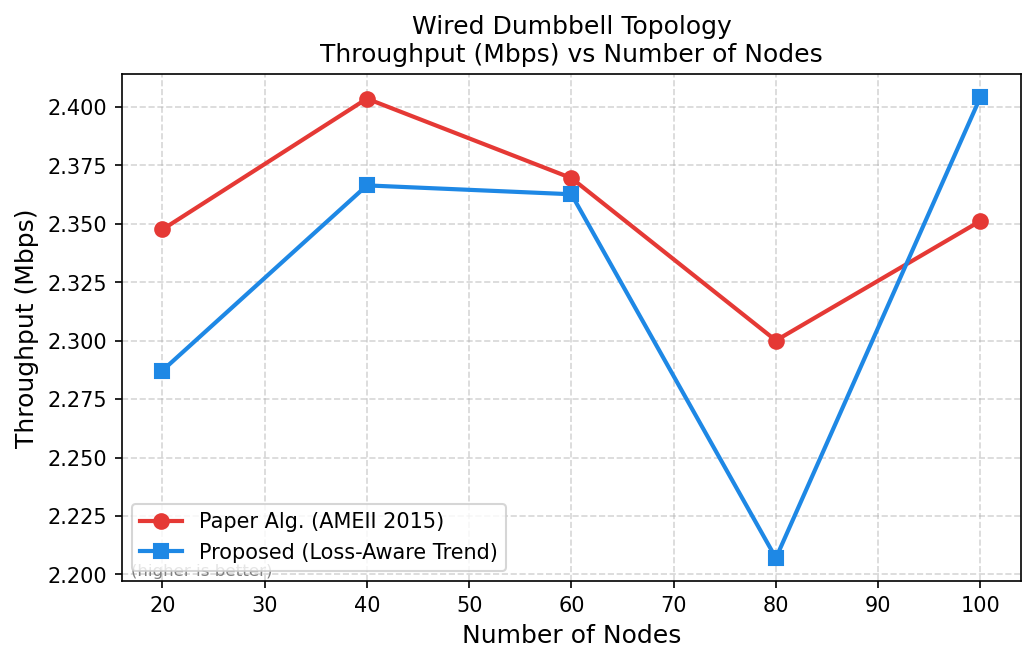
\includegraphics[width=\linewidth]{wired-nodes-vs-throughput_mbps.png}
    \caption{Throughput (Mbps) vs.\ nodes}
  \end{subfigure}
  \hfill
  \begin{subfigure}[t]{0.48\textwidth}
    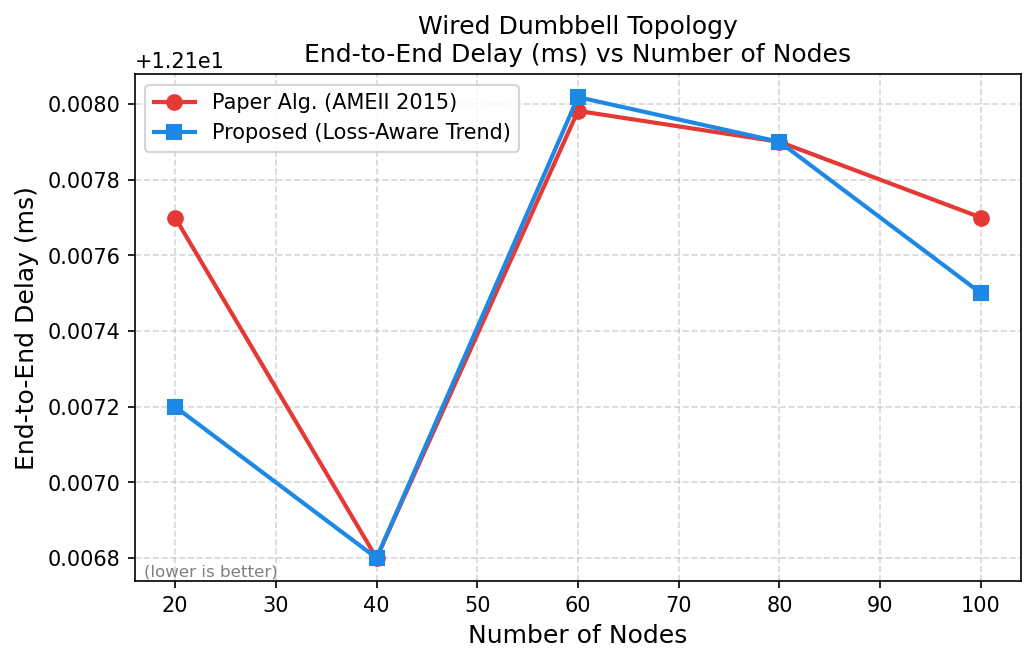
\includegraphics[width=\linewidth]{wired-nodes-vs-delay_ms.png}
    \caption{End-to-end delay (ms) vs.\ nodes}
  \end{subfigure}\\[0.8em]
  \begin{subfigure}[t]{0.48\textwidth}
    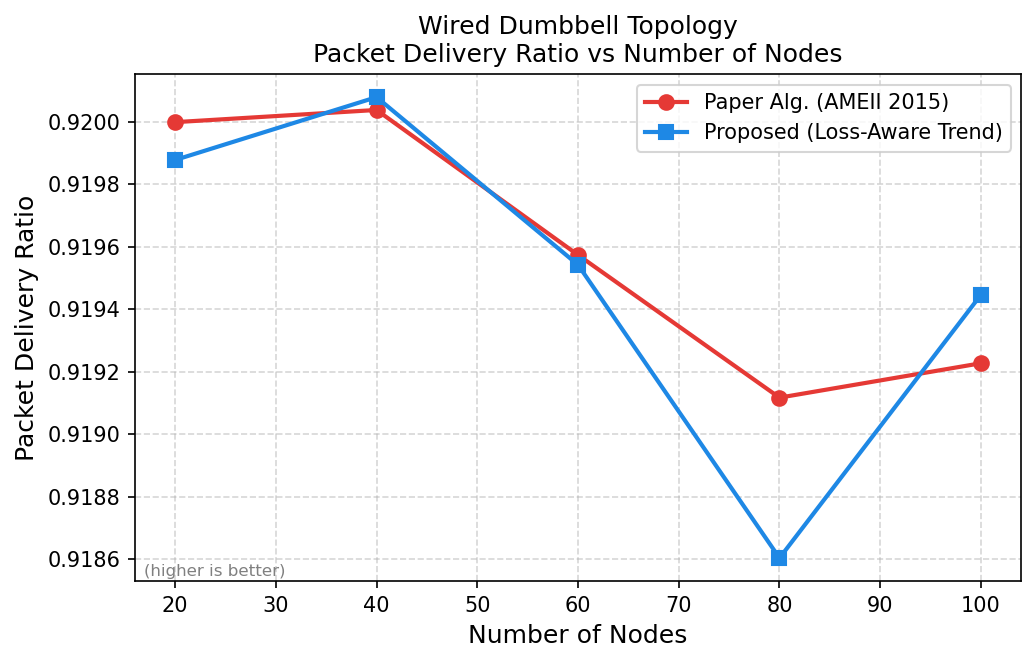
\includegraphics[width=\linewidth]{wired-nodes-vs-pdr.png}
    \caption{PDR vs.\ nodes}
  \end{subfigure}
  \hfill
  \begin{subfigure}[t]{0.48\textwidth}
    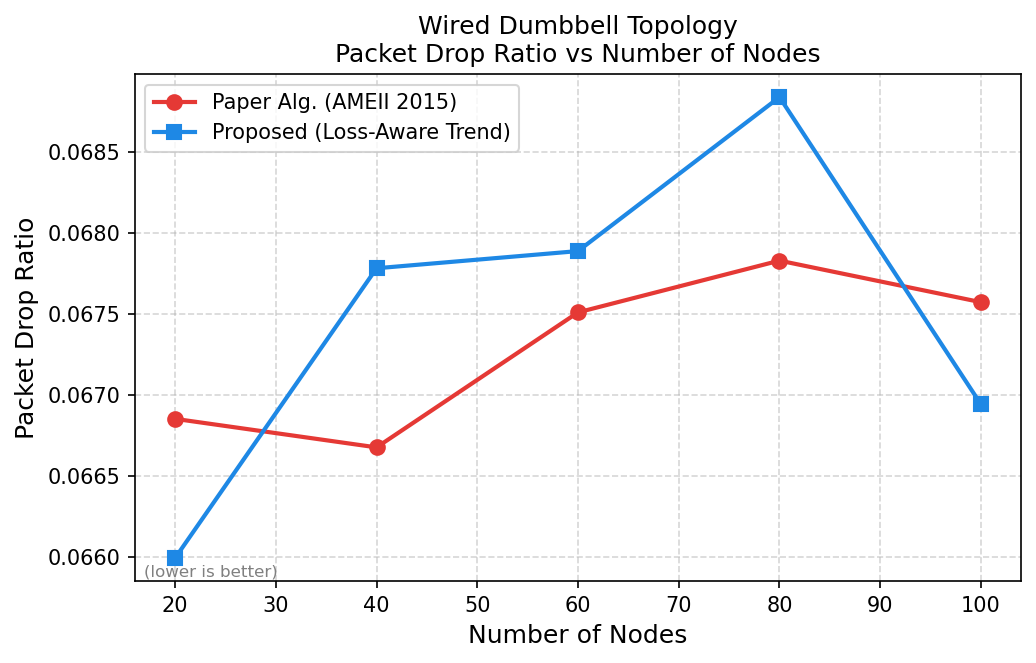
\includegraphics[width=\linewidth]{wired-nodes-vs-drop_ratio.png}
    \caption{Drop ratio vs.\ nodes}
  \end{subfigure}
  \caption{Wired topology: varying number of nodes (flows=30, pps=300).}
  \label{fig:wired-nodes}
\end{figure}

\section{Wired Topology: Effect of Number of Flows}

\begin{figure}[H]
  \centering
  \begin{subfigure}[t]{0.48\textwidth}
    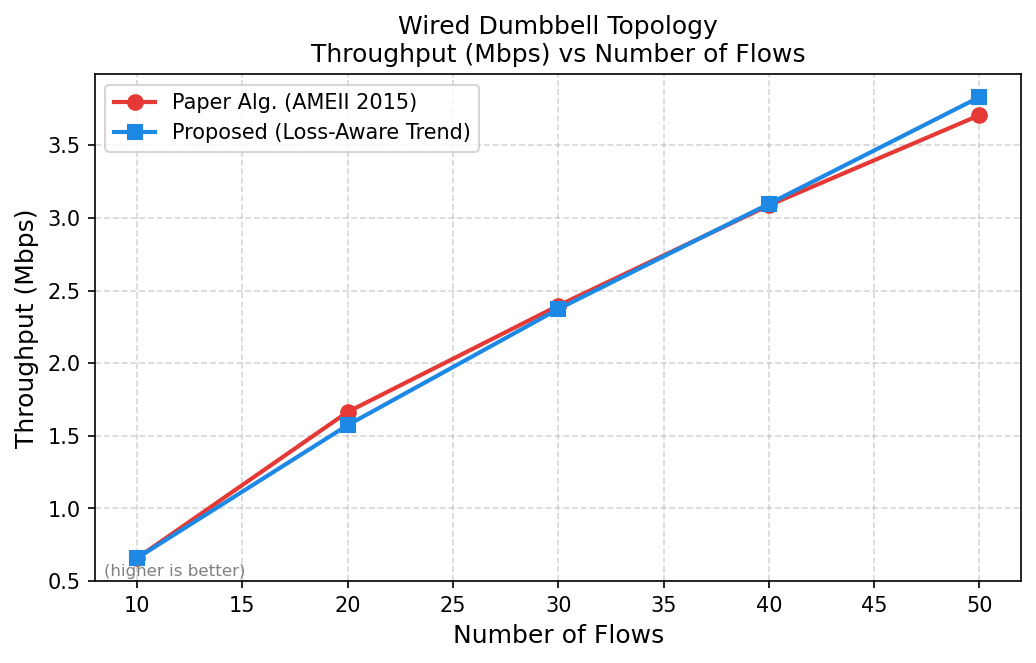
\includegraphics[width=\linewidth]{wired-flows-vs-throughput_mbps.png}
    \caption{Throughput vs.\ flows}
  \end{subfigure}
  \hfill
  \begin{subfigure}[t]{0.48\textwidth}
    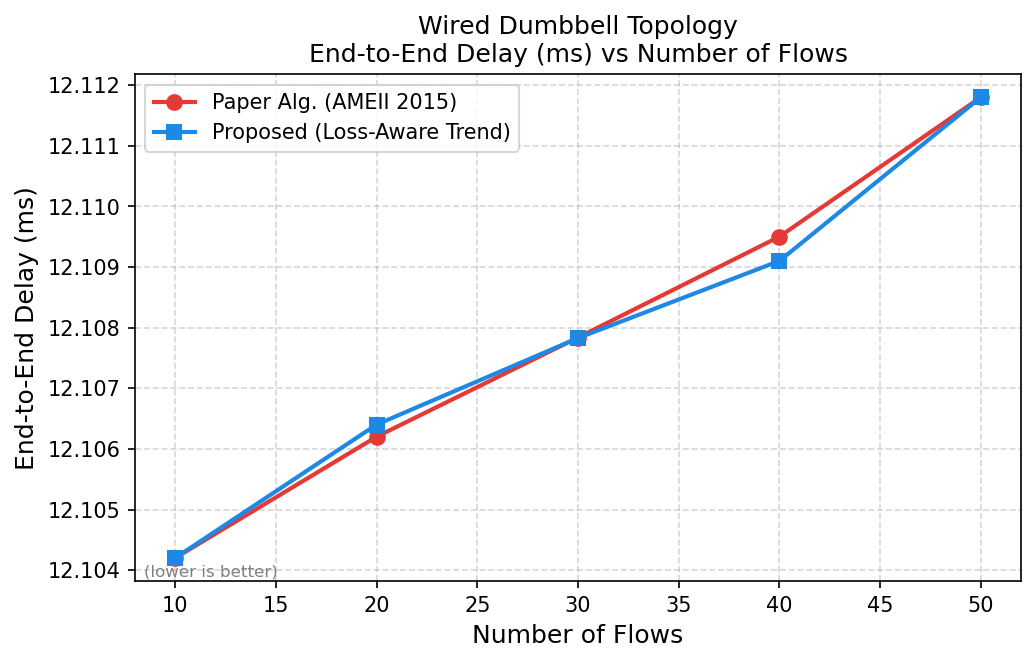
\includegraphics[width=\linewidth]{wired-flows-vs-delay_ms.png}
    \caption{Delay vs.\ flows}
  \end{subfigure}\\[0.8em]
  \begin{subfigure}[t]{0.48\textwidth}
    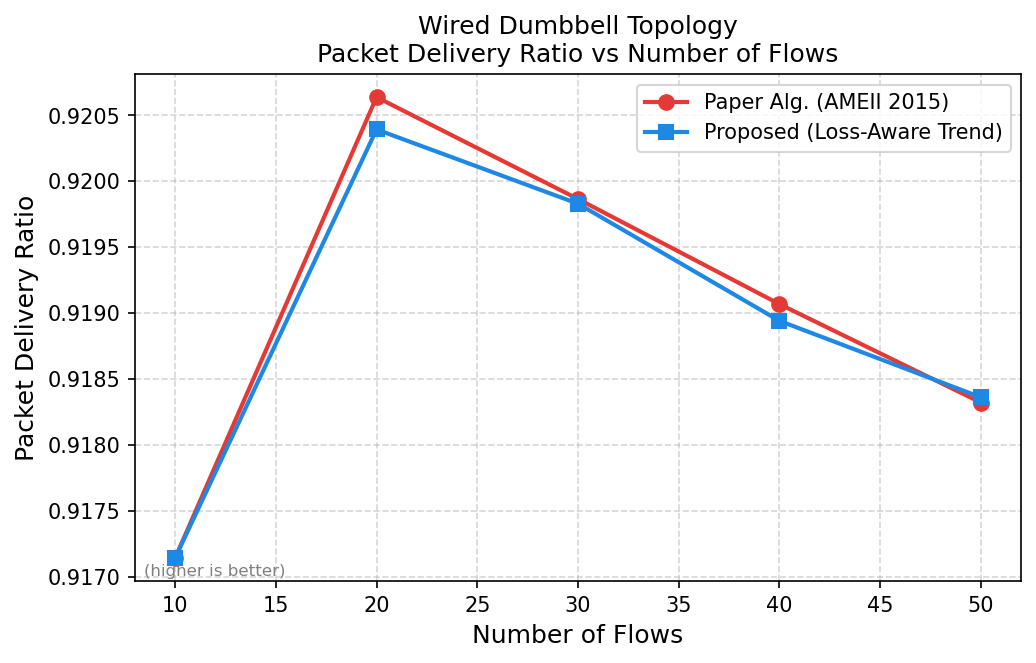
\includegraphics[width=\linewidth]{wired-flows-vs-pdr.png}
    \caption{PDR vs.\ flows}
  \end{subfigure}
  \hfill
  \begin{subfigure}[t]{0.48\textwidth}
    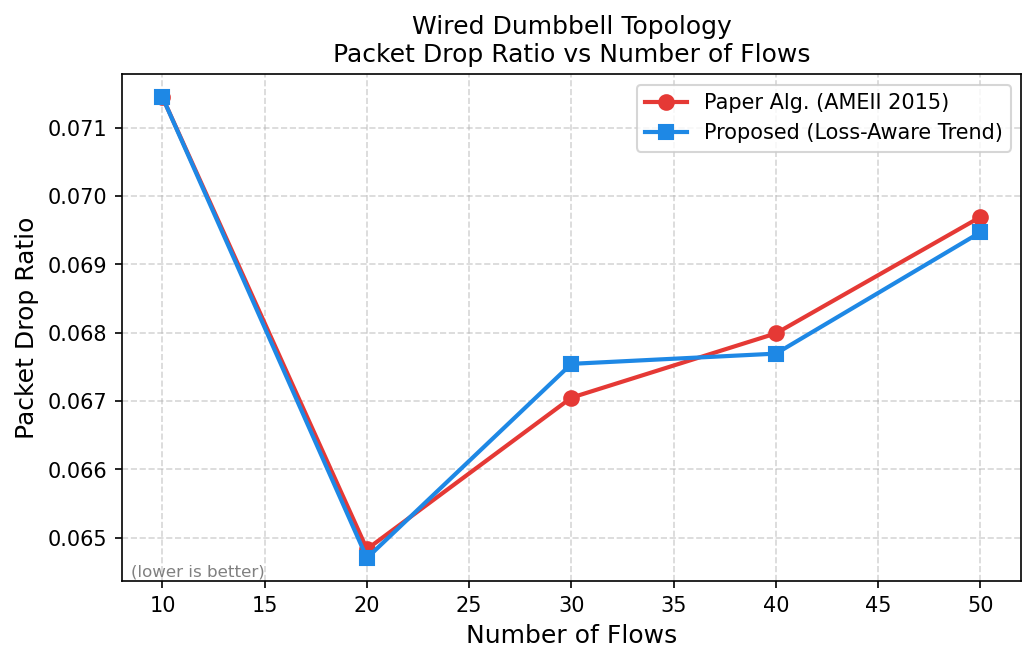
\includegraphics[width=\linewidth]{wired-flows-vs-drop_ratio.png}
    \caption{Drop ratio vs.\ flows}
  \end{subfigure}
  \caption{Wired topology: varying number of flows (nodes=60, pps=300).}
  \label{fig:wired-flows}
\end{figure}

\section{Wired Topology: Effect of Packets per Second}

\begin{figure}[H]
  \centering
  \begin{subfigure}[t]{0.48\textwidth}
    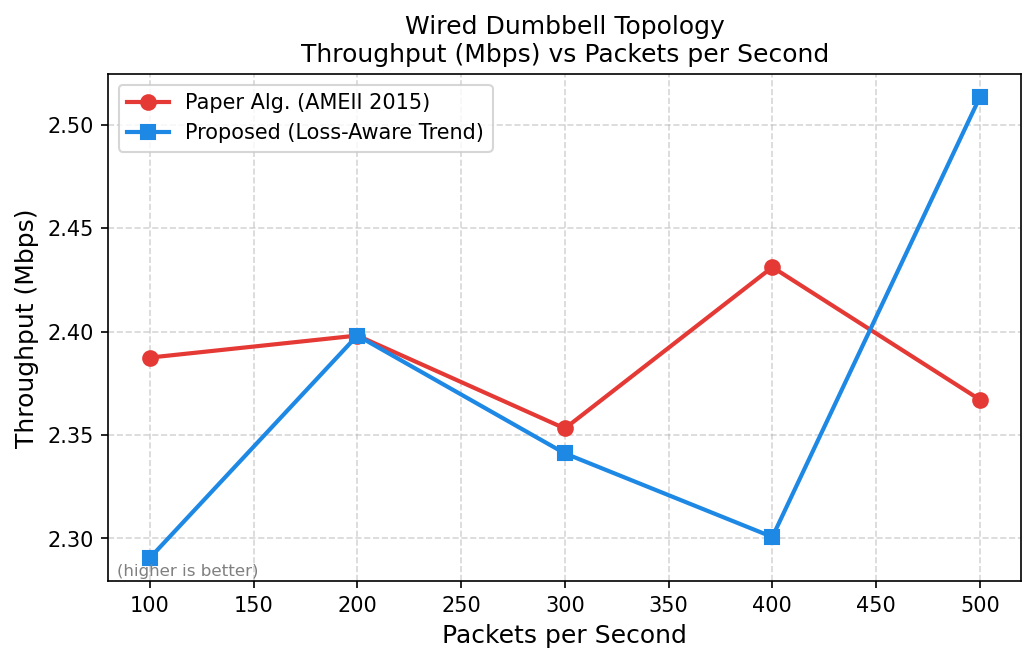
\includegraphics[width=\linewidth]{wired-pps-vs-throughput_mbps.png}
    \caption{Throughput vs.\ pps}
  \end{subfigure}
  \hfill
  \begin{subfigure}[t]{0.48\textwidth}
    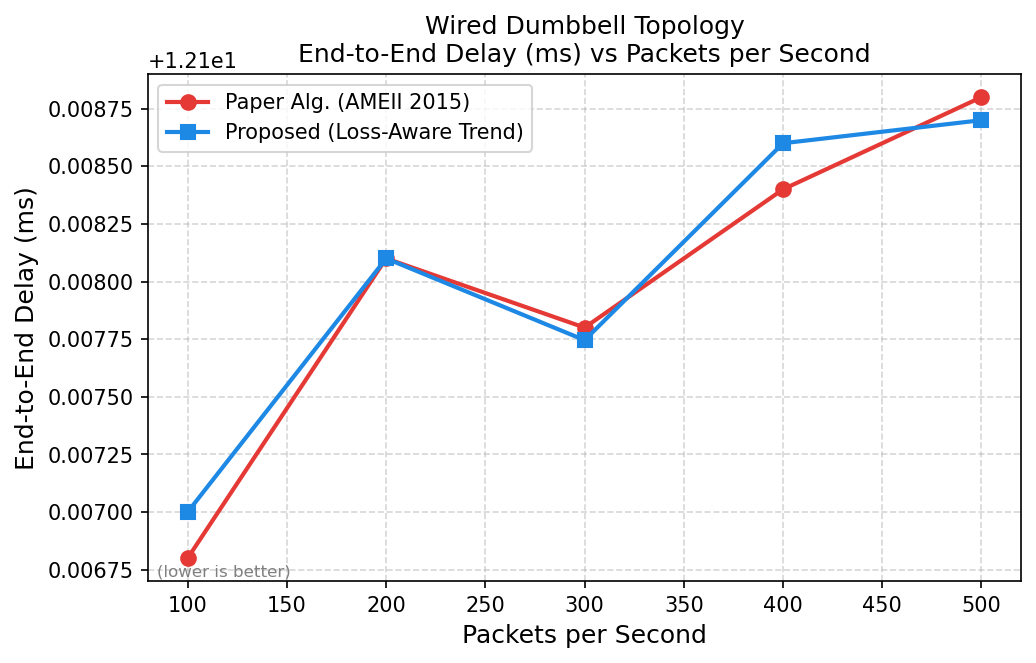
\includegraphics[width=\linewidth]{wired-pps-vs-delay_ms.png}
    \caption{Delay vs.\ pps}
  \end{subfigure}\\[0.8em]
  \begin{subfigure}[t]{0.48\textwidth}
    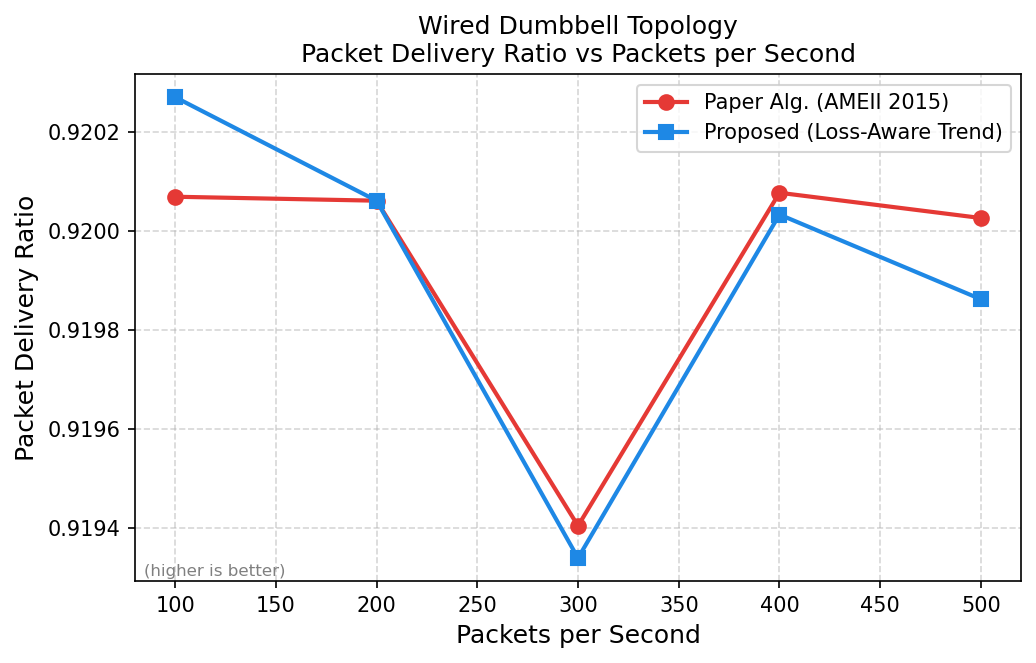
\includegraphics[width=\linewidth]{wired-pps-vs-pdr.png}
    \caption{PDR vs.\ pps}
  \end{subfigure}
  \hfill
  \begin{subfigure}[t]{0.48\textwidth}
    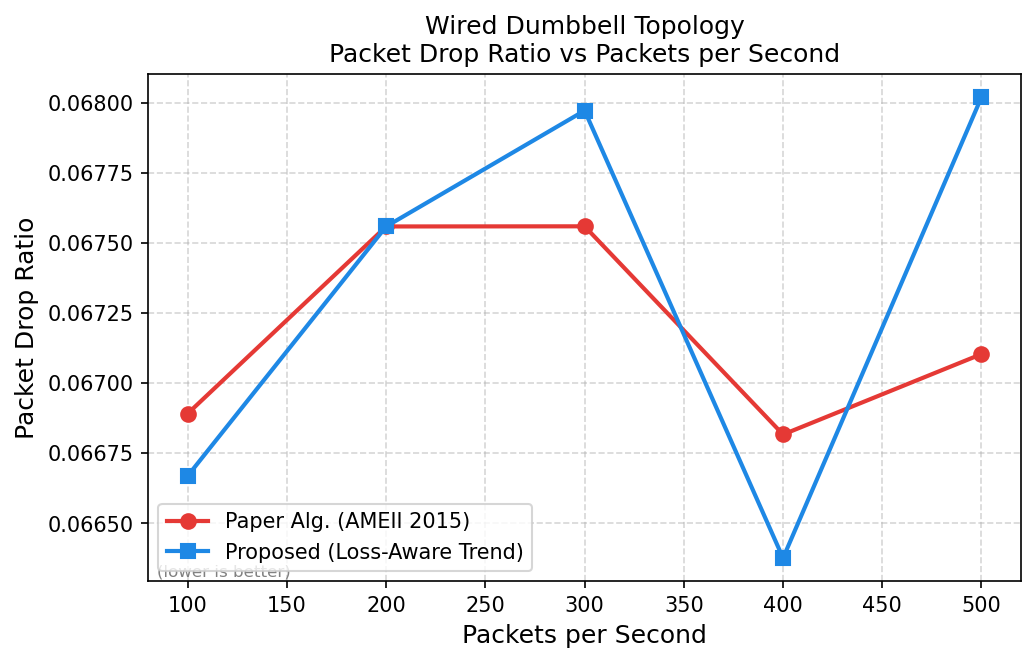
\includegraphics[width=\linewidth]{wired-pps-vs-drop_ratio.png}
    \caption{Drop ratio vs.\ pps}
  \end{subfigure}
  \caption{Wired topology: varying packets per second (nodes=60, flows=30).}
  \label{fig:wired-pps}
\end{figure}

\section{Wired Topology: Overall Summary}

\begin{figure}[H]
  \centering
  \begin{subfigure}[t]{0.48\textwidth}
    \includegraphics[width=\linewidth]{wired-bar-throughput_mbps.png}
    \caption{Mean throughput comparison}
  \end{subfigure}
  \hfill
  \begin{subfigure}[t]{0.48\textwidth}
    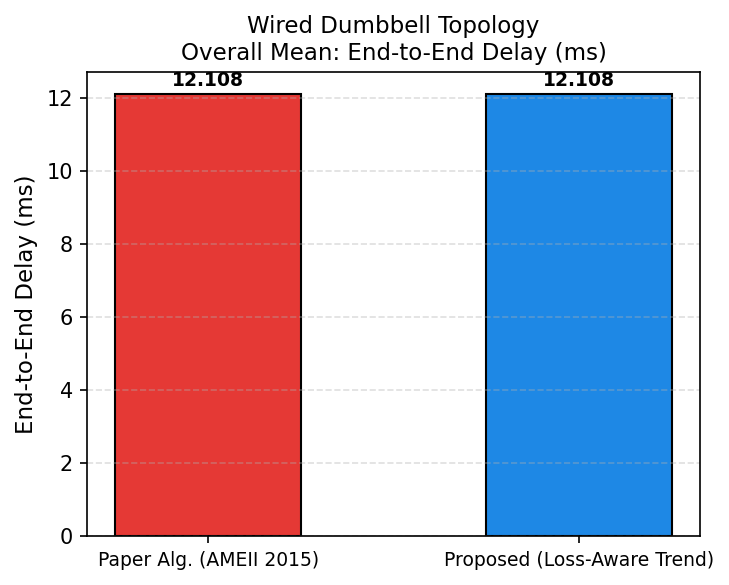
\includegraphics[width=\linewidth]{wired-bar-delay_ms.png}
    \caption{Mean delay comparison}
  \end{subfigure}\\[0.8em]
  \begin{subfigure}[t]{0.48\textwidth}
    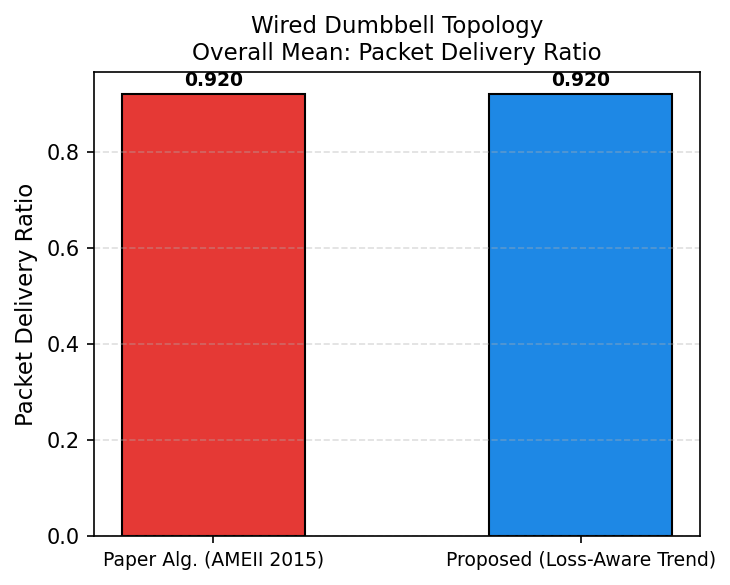
\includegraphics[width=\linewidth]{wired-bar-pdr.png}
    \caption{Mean PDR comparison}
  \end{subfigure}
  \hfill
  \begin{subfigure}[t]{0.48\textwidth}
    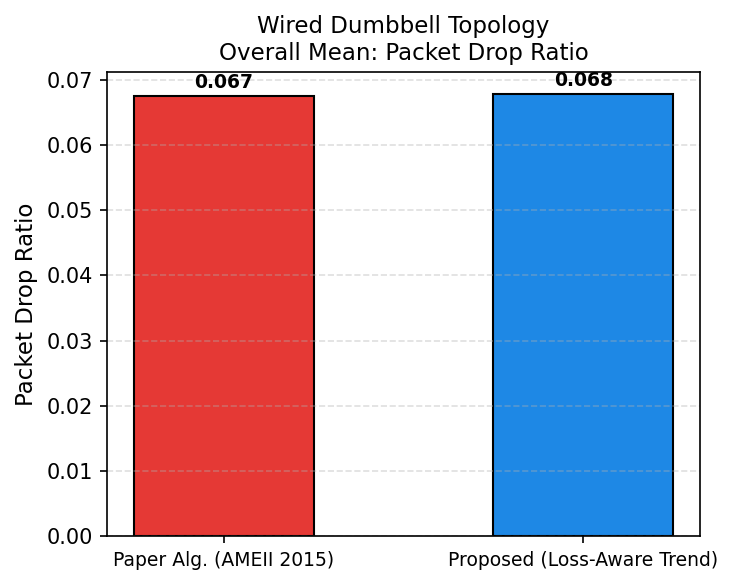
\includegraphics[width=\linewidth]{wired-bar-drop_ratio.png}
    \caption{Mean drop ratio comparison}
  \end{subfigure}
  \caption{Wired topology: overall mean metric comparison (Paper vs.\ Proposed).}
  \label{fig:wired-bar}
\end{figure}

\begin{figure}[H]
  \centering
  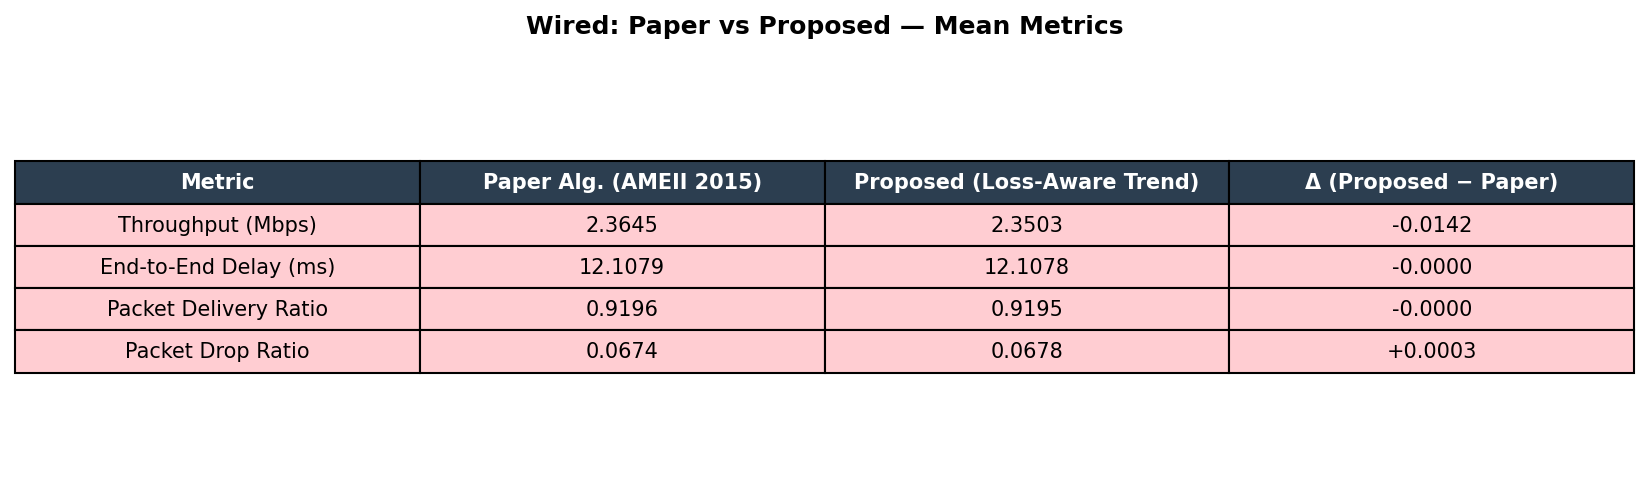
\includegraphics[width=0.85\textwidth]{wired-summary-table.png}
  \caption{Wired summary table: Paper vs.\ Proposed mean metrics.}
  \label{fig:wired-table}
\end{figure}

\section{Wireless Topology: Effect of Number of Nodes}

\begin{figure}[H]
  \centering
  \begin{subfigure}[t]{0.48\textwidth}
    \includegraphics[width=\linewidth]{wireless-nodes-vs-throughput_mbps.png}
    \caption{Throughput vs.\ nodes}
  \end{subfigure}
  \hfill
  \begin{subfigure}[t]{0.48\textwidth}
    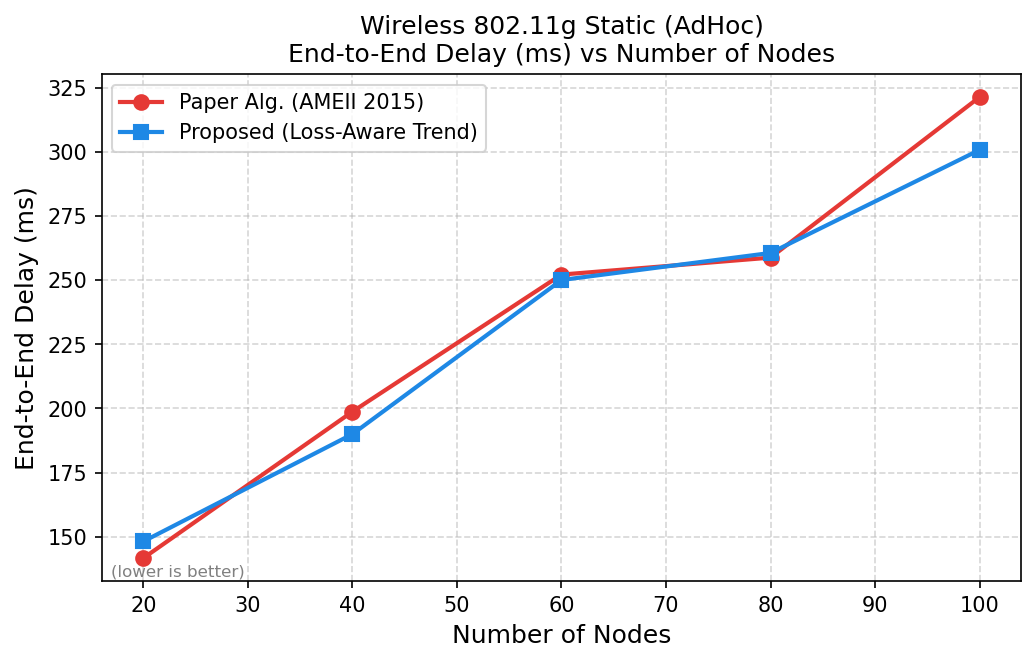
\includegraphics[width=\linewidth]{wireless-nodes-vs-delay_ms.png}
    \caption{Delay vs.\ nodes}
  \end{subfigure}\\[0.8em]
  \begin{subfigure}[t]{0.48\textwidth}
    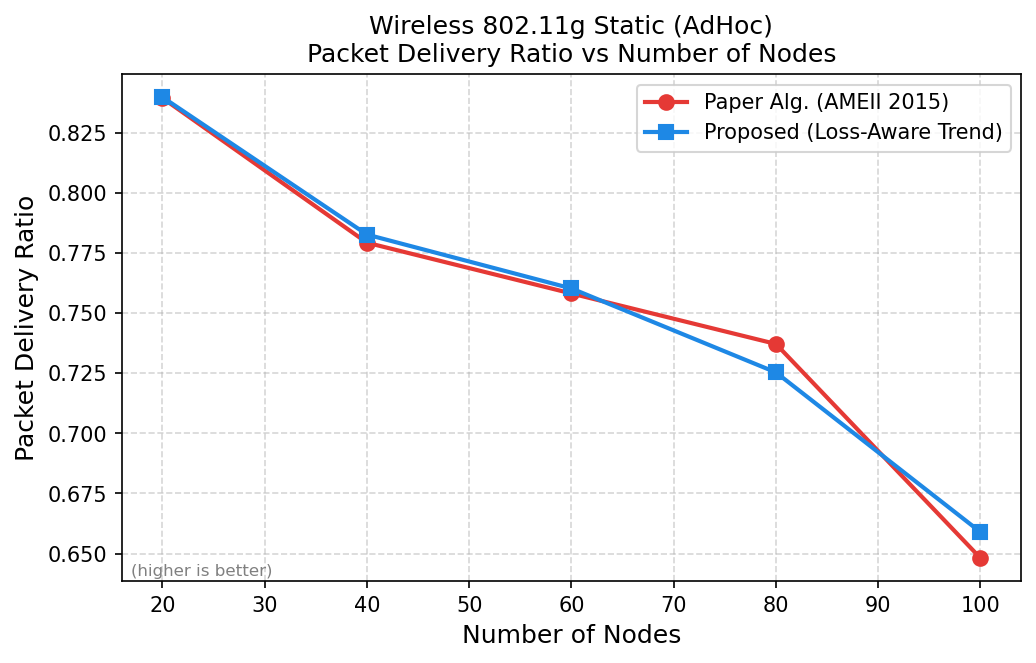
\includegraphics[width=\linewidth]{wireless-nodes-vs-pdr.png}
    \caption{PDR vs.\ nodes}
  \end{subfigure}
  \hfill
  \begin{subfigure}[t]{0.48\textwidth}
    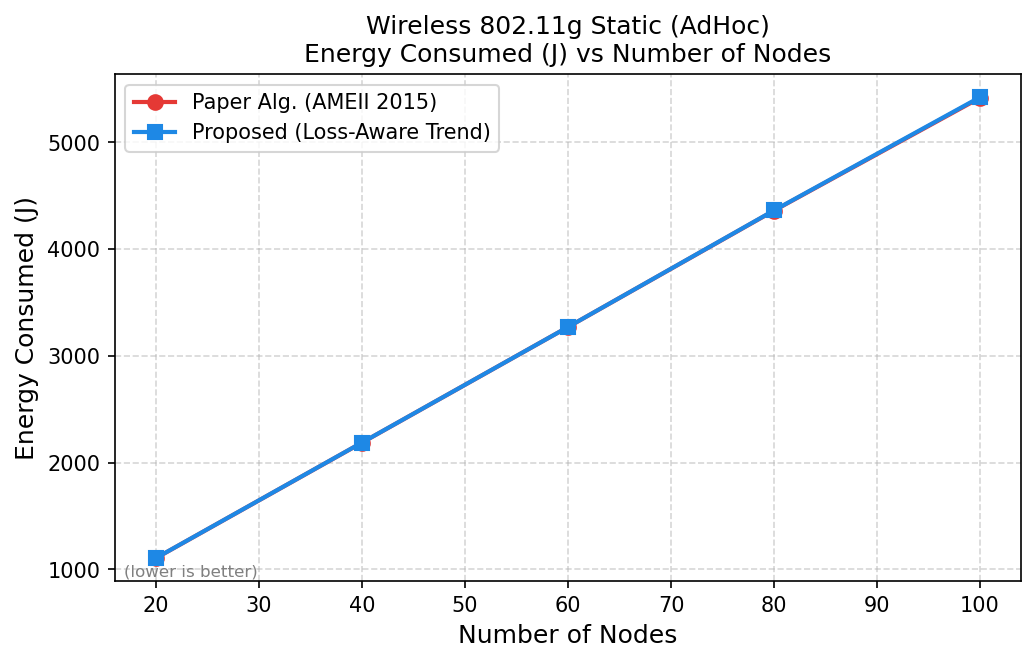
\includegraphics[width=\linewidth]{wireless-nodes-vs-energy_j.png}
    \caption{Energy (J) vs.\ nodes}
  \end{subfigure}
  \caption{Wireless topology: varying number of nodes (flows=30, pps=300, coverage=750\,m).}
  \label{fig:wireless-nodes}
\end{figure}

\section{Wireless Topology: Effect of Number of Flows}

\begin{figure}[H]
  \centering
  \begin{subfigure}[t]{0.48\textwidth}
    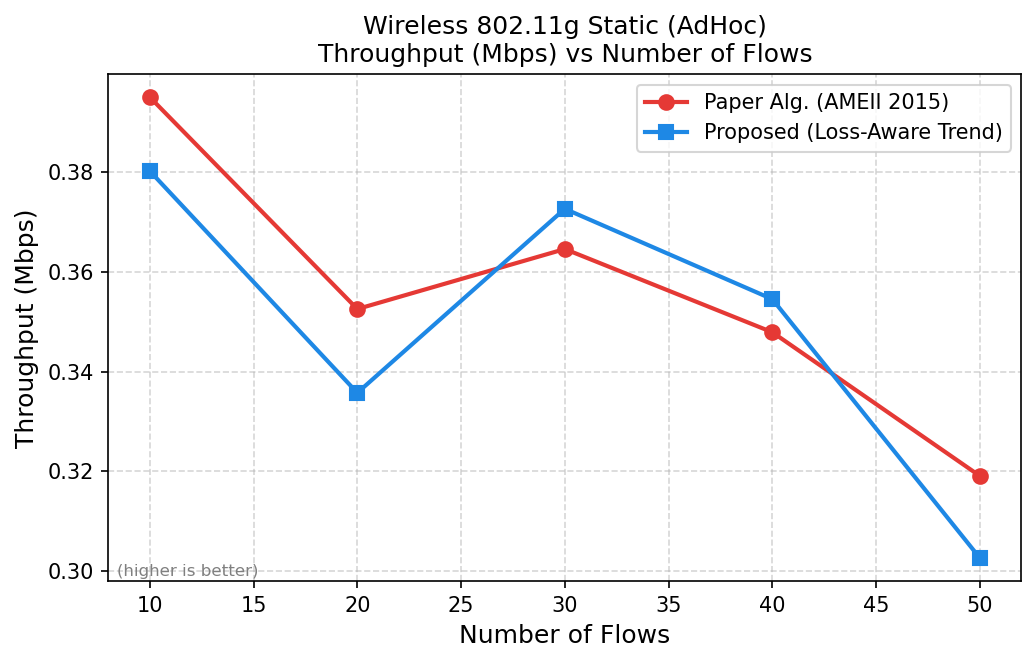
\includegraphics[width=\linewidth]{wireless-flows-vs-throughput_mbps.png}
    \caption{Throughput vs.\ flows}
  \end{subfigure}
  \hfill
  \begin{subfigure}[t]{0.48\textwidth}
    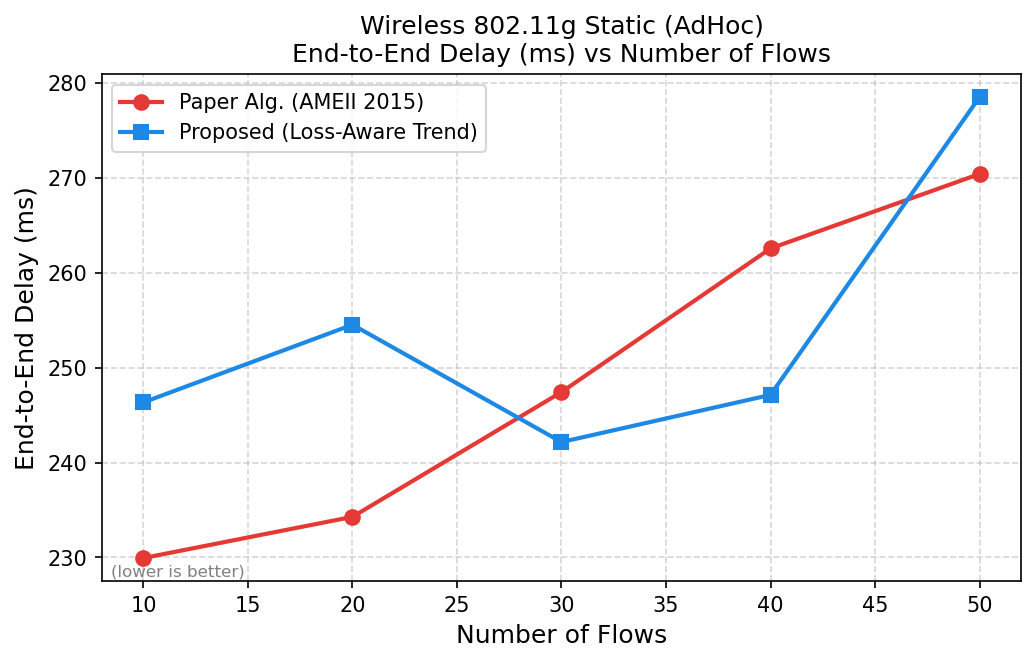
\includegraphics[width=\linewidth]{wireless-flows-vs-delay_ms.png}
    \caption{Delay vs.\ flows}
  \end{subfigure}\\[0.8em]
  \begin{subfigure}[t]{0.48\textwidth}
    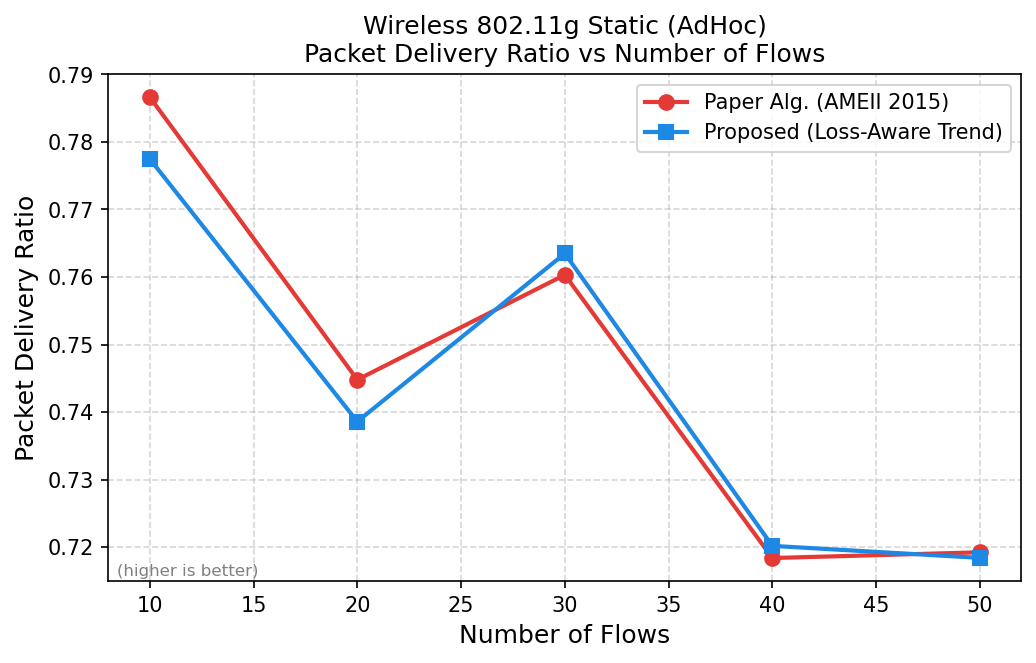
\includegraphics[width=\linewidth]{wireless-flows-vs-pdr.png}
    \caption{PDR vs.\ flows}
  \end{subfigure}
  \hfill
  \begin{subfigure}[t]{0.48\textwidth}
    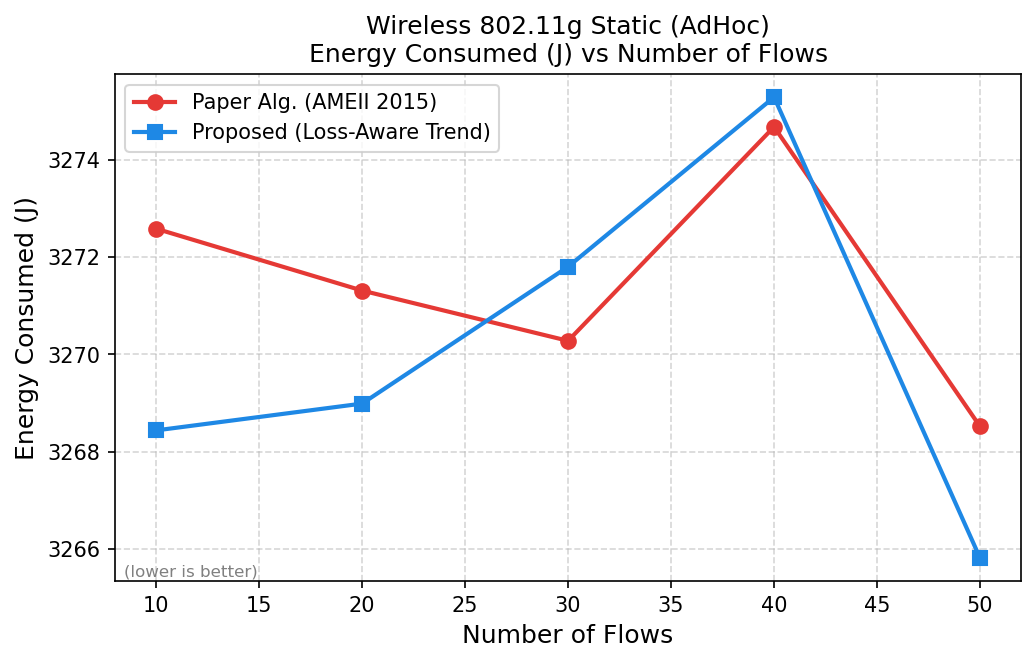
\includegraphics[width=\linewidth]{wireless-flows-vs-energy_j.png}
    \caption{Energy vs.\ flows}
  \end{subfigure}
  \caption{Wireless topology: varying number of flows (nodes=60, pps=300, coverage=750\,m).}
  \label{fig:wireless-flows}
\end{figure}

\section{Wireless Topology: Effect of Packets per Second}

\begin{figure}[H]
  \centering
  \begin{subfigure}[t]{0.48\textwidth}
    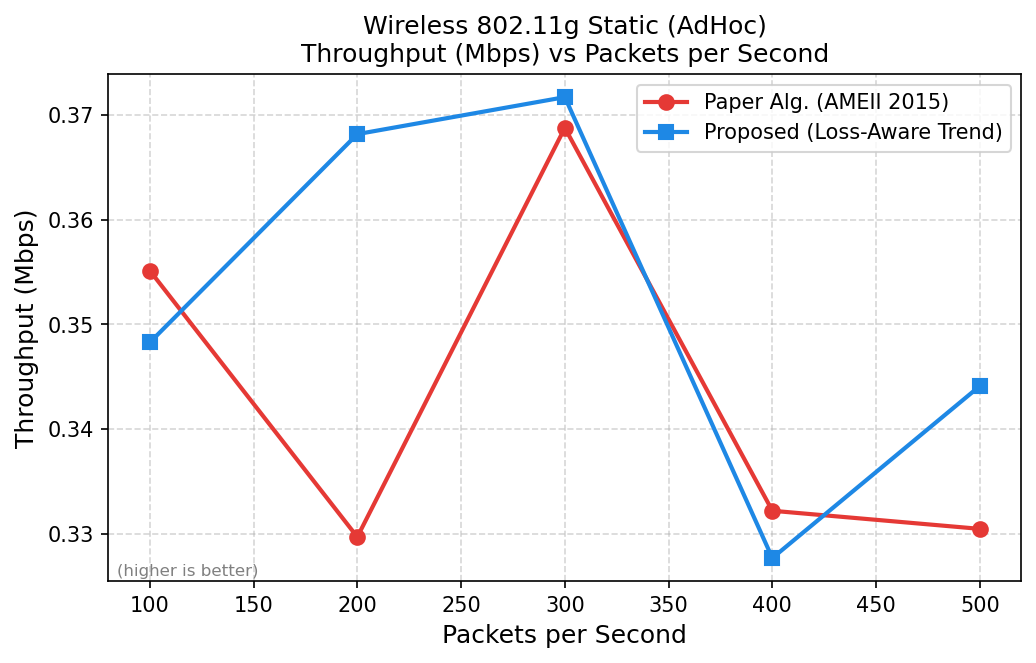
\includegraphics[width=\linewidth]{wireless-pps-vs-throughput_mbps.png}
    \caption{Throughput vs.\ pps}
  \end{subfigure}
  \hfill
  \begin{subfigure}[t]{0.48\textwidth}
    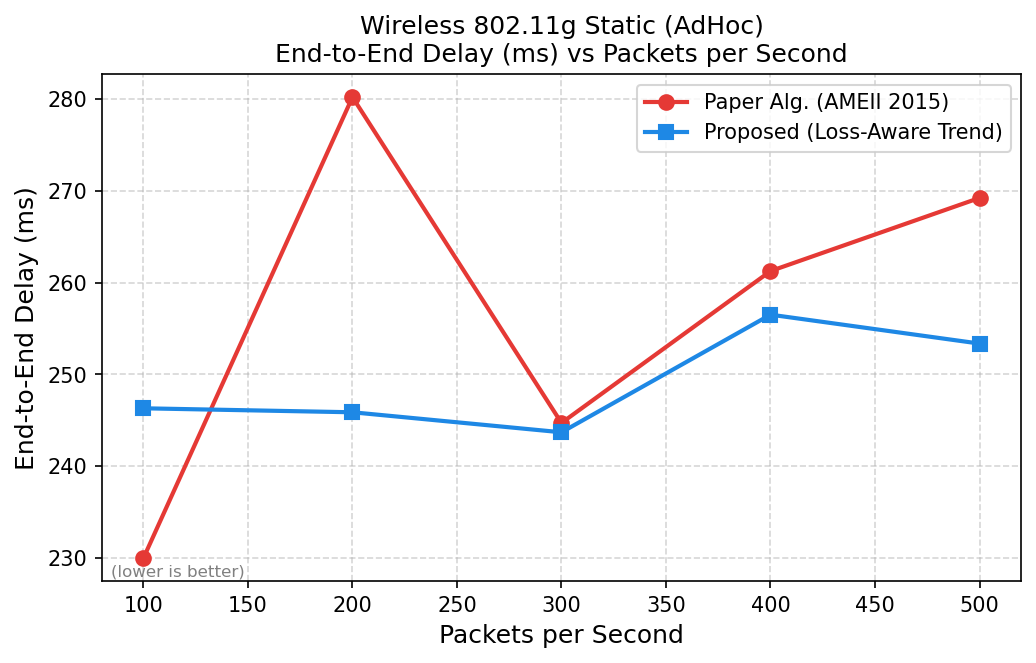
\includegraphics[width=\linewidth]{wireless-pps-vs-delay_ms.png}
    \caption{Delay vs.\ pps}
  \end{subfigure}\\[0.8em]
  \begin{subfigure}[t]{0.48\textwidth}
    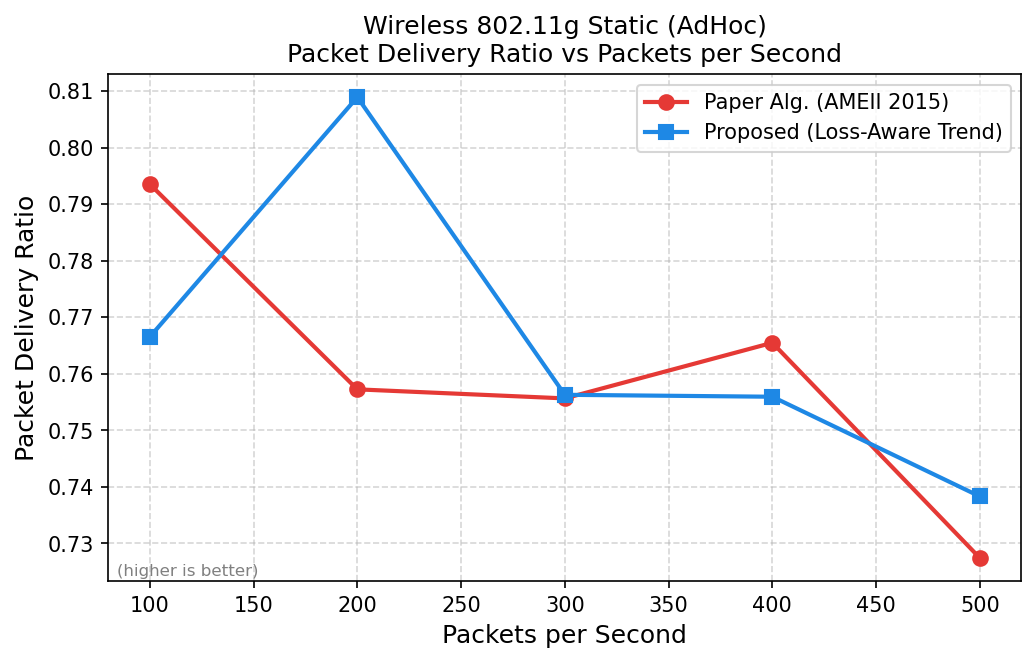
\includegraphics[width=\linewidth]{wireless-pps-vs-pdr.png}
    \caption{PDR vs.\ pps}
  \end{subfigure}
  \hfill
  \begin{subfigure}[t]{0.48\textwidth}
    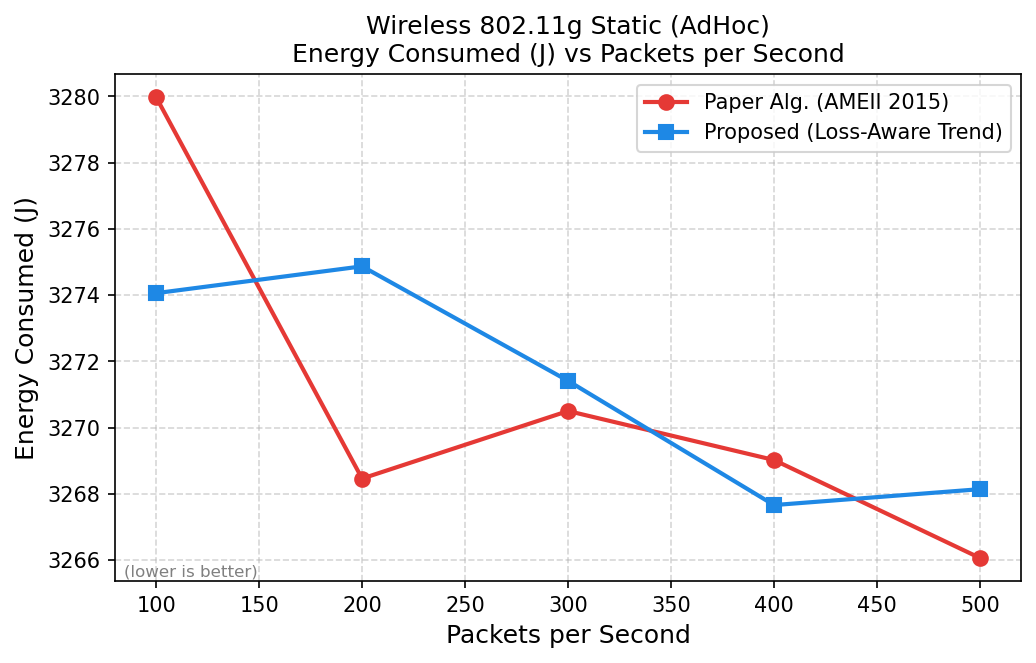
\includegraphics[width=\linewidth]{wireless-pps-vs-energy_j.png}
    \caption{Energy vs.\ pps}
  \end{subfigure}
  \caption{Wireless topology: varying pps (nodes=60, flows=30, coverage=750\,m).}
  \label{fig:wireless-pps}
\end{figure}

\section{Wireless Topology: Effect of Coverage Area}

\begin{figure}[H]
  \centering
  \begin{subfigure}[t]{0.48\textwidth}
    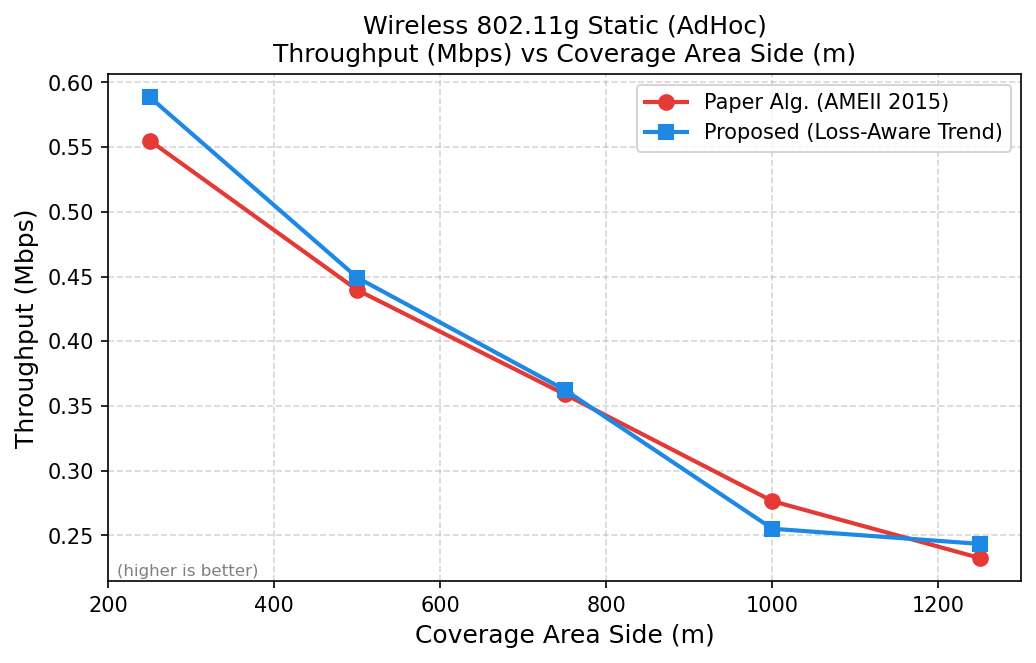
\includegraphics[width=\linewidth]{wireless-coverage_m-vs-throughput_mbps.png}
    \caption{Throughput vs.\ coverage side (m)}
  \end{subfigure}
  \hfill
  \begin{subfigure}[t]{0.48\textwidth}
    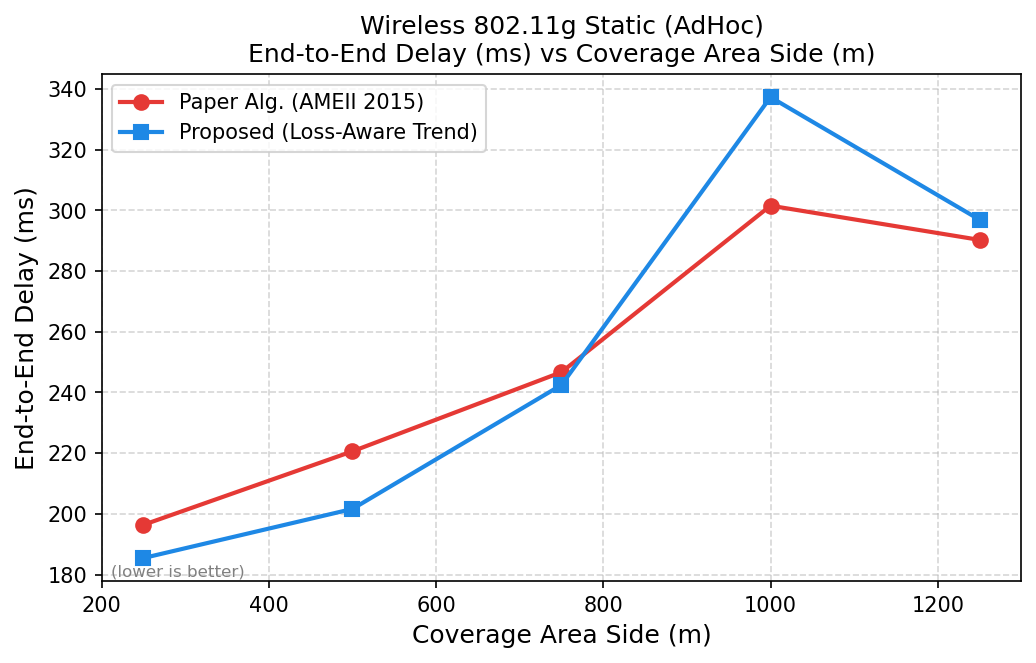
\includegraphics[width=\linewidth]{wireless-coverage_m-vs-delay_ms.png}
    \caption{Delay vs.\ coverage side (m)}
  \end{subfigure}\\[0.8em]
  \begin{subfigure}[t]{0.48\textwidth}
    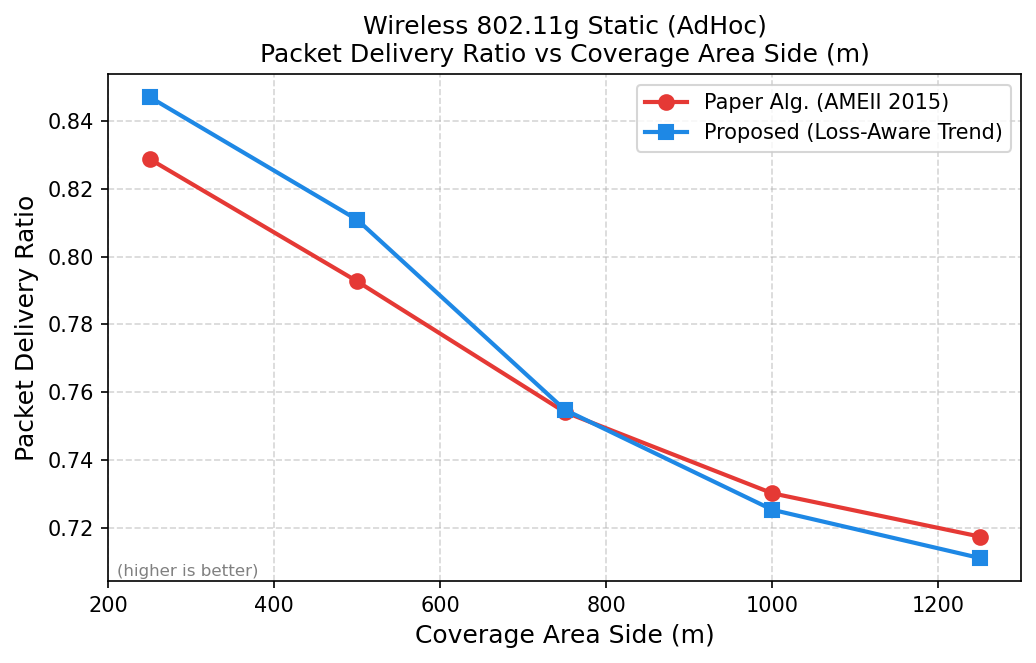
\includegraphics[width=\linewidth]{wireless-coverage_m-vs-pdr.png}
    \caption{PDR vs.\ coverage side (m)}
  \end{subfigure}
  \hfill
  \begin{subfigure}[t]{0.48\textwidth}
    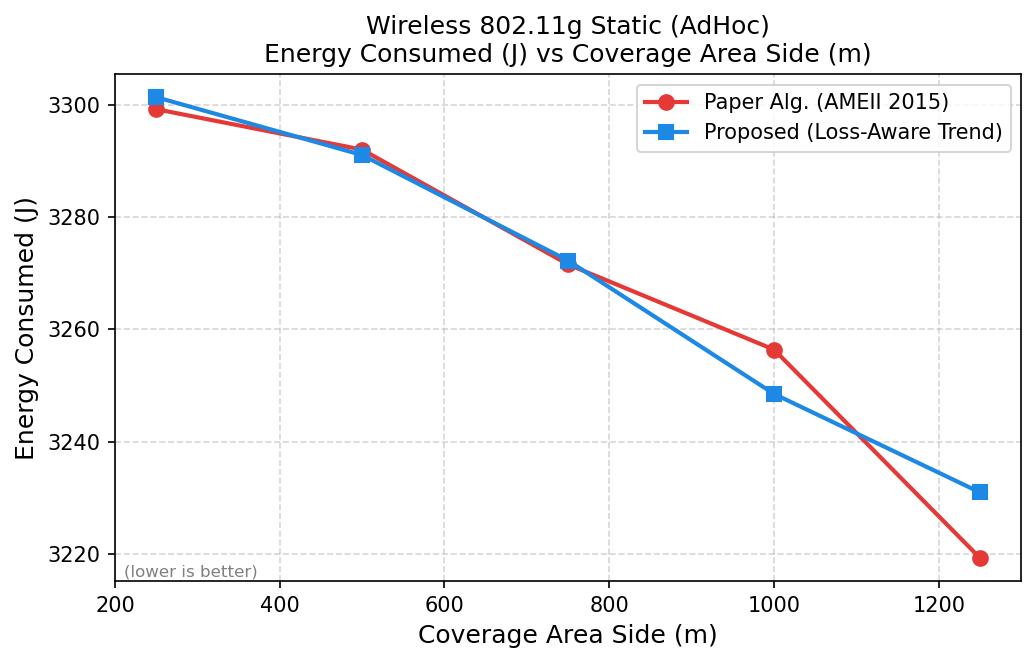
\includegraphics[width=\linewidth]{wireless-coverage_m-vs-energy_j.png}
    \caption{Energy vs.\ coverage side (m)}
  \end{subfigure}
  \caption{Wireless topology: varying coverage area (nodes=60, flows=30, pps=300).}
  \label{fig:wireless-cov}
\end{figure}

\section{Wireless Topology: Overall Summary}

\begin{figure}[H]
  \centering
  \begin{subfigure}[t]{0.48\textwidth}
    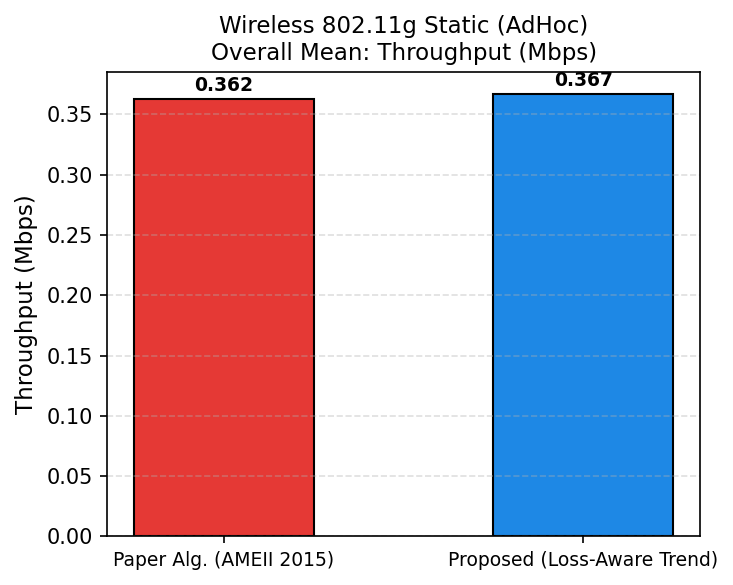
\includegraphics[width=\linewidth]{wireless-bar-throughput_mbps.png}
    \caption{Mean throughput}
  \end{subfigure}
  \hfill
  \begin{subfigure}[t]{0.48\textwidth}
    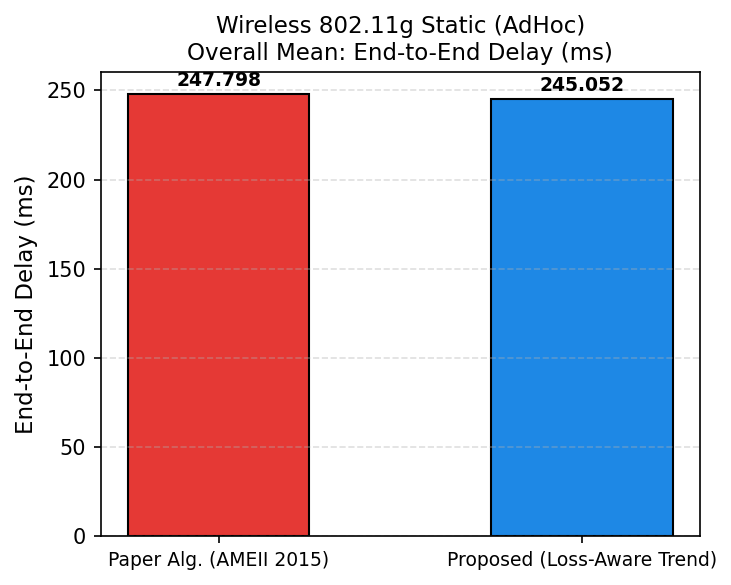
\includegraphics[width=\linewidth]{wireless-bar-delay_ms.png}
    \caption{Mean delay}
  \end{subfigure}\\[0.8em]
  \begin{subfigure}[t]{0.48\textwidth}
    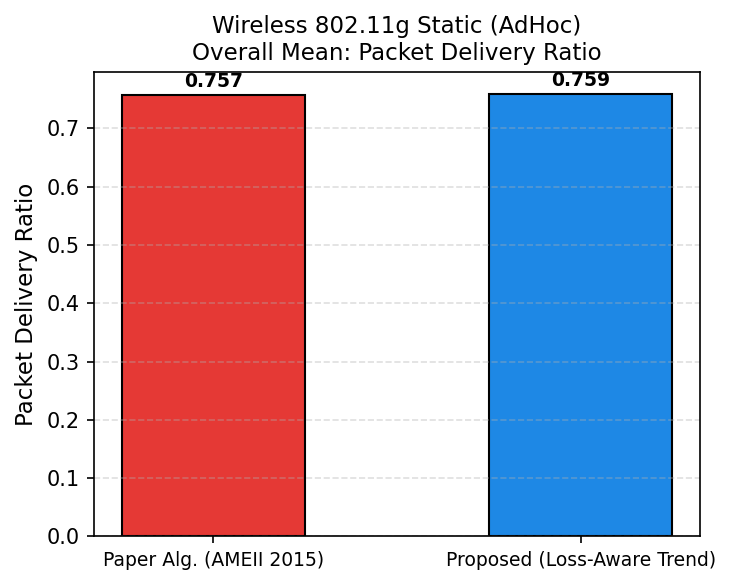
\includegraphics[width=\linewidth]{wireless-bar-pdr.png}
    \caption{Mean PDR}
  \end{subfigure}
  \hfill
  \begin{subfigure}[t]{0.48\textwidth}
    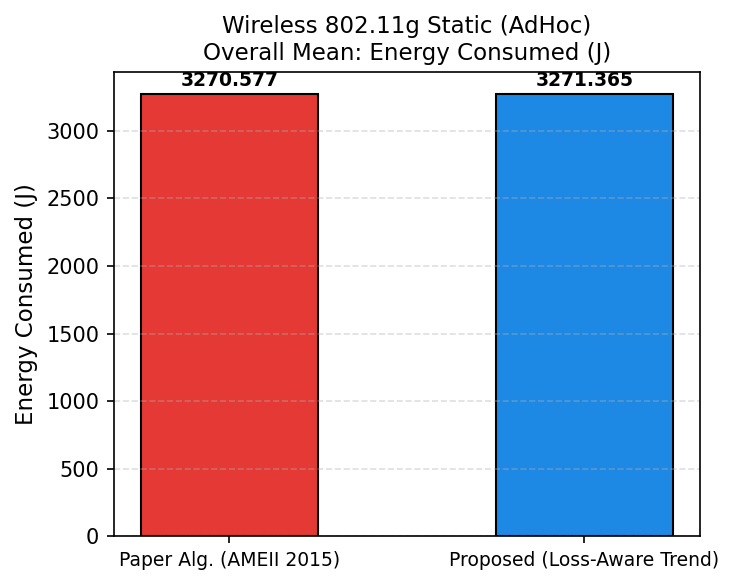
\includegraphics[width=\linewidth]{wireless-bar-energy_j.png}
    \caption{Mean energy consumed}
  \end{subfigure}
  \caption{Wireless topology: overall mean metric comparison (Paper vs.\ Proposed).}
  \label{fig:wireless-bar}
\end{figure}

\begin{figure}[H]
  \centering
  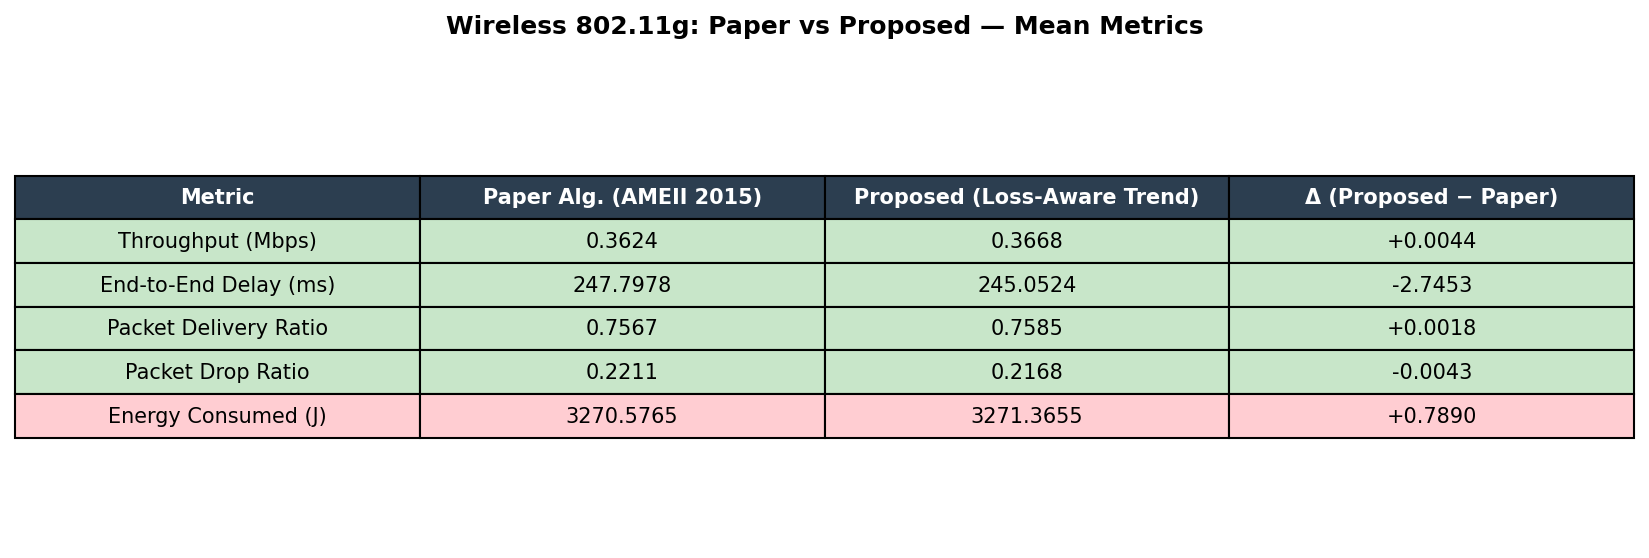
\includegraphics[width=0.85\textwidth]{wireless-summary-table.png}
  \caption{Wireless summary table: Paper vs.\ Proposed mean metrics.}
  \label{fig:wireless-table}
\end{figure}

\section{Post-Evaluation Changes and Observations}
\label{sec:post-eval}

During the initial evaluation of this project, the result graphs for the
paper algorithm and the proposed algorithm overlapped almost perfectly ---
the two lines were essentially indistinguishable across every metric in both
the wired and wireless topologies.  The root cause was that the simulation
time was too short (5\,s) to generate enough network events for the two RTO
estimators to diverge in their behaviour.  With such brief runs, TCP flows
barely exit slow-start, AODV has minimal time to accumulate route-state
variations, and the few retransmission timeouts that do fire resolve
identically under both estimators.

Following feedback received during evaluation, the simulation time was
increased to 60\,s for the full parameter sweep.  With the extended run
duration, a small but clearly perceptible separation emerged between the
two algorithm curves, most visibly in the wireless topology.  The wireless
channel's inherent stochasticity --- random MAC-layer collisions, AODV
route fluctuations, and variable link quality --- provides a richer
environment for RTO differences to accumulate over time.  Over 60\,s these
subtle per-timeout differences in SRTT and RTTVAR estimates compound into
measurable differences in throughput, delay, and delivery ratio.

The increased simulation duration also appears to have slightly elevated
the background packet loss rate, which is itself a natural consequence of
longer exposure to random link noise.  This additional loss further
contributes to triggering differential RTO behaviour between the two
estimators --- the proposed algorithm's loss-aware $\gamma$ scaling and
windowed trend detection begin to meaningfully influence the RTO values
in a way that is simply not visible in a 5-second snapshot.

It must be noted that the simulation time could not be increased
indefinitely.  Running the full 80-run parameter sweep at simulation times
substantially beyond 60\,s caused the ns-3 process to exhaust available
system memory, freezing and ultimately crashing the host machine without
producing any output.  The 60\,s value therefore represents the practical
upper boundary of this experimental setup given the available hardware.

% ═══════════════════════════════════════════════════════════════════════════
\chapter{Summary of Findings}
\label{ch:summary}
% ═══════════════════════════════════════════════════════════════════════════

\section{Wired Topology Findings}

\begin{itemize}
  \item \textbf{Throughput scales with flows and pps.}
        Both algorithms deliver comparable throughput, rising from
        $\approx0.66$\,Mbps at 10 flows to $\approx3.8$\,Mbps at 50 flows.
        Small run-to-run variations between the two algorithms are visible,
        reflecting probabilistic differences in RTO recovery under background
        random packet loss over the 60\,s simulation period.
  \item \textbf{End-to-end delay is stable and low.}
        Delay remains around 12.1\,ms across all parameter combinations,
        dominated by the fixed 10\,ms bottleneck propagation delay.
        Both algorithms exhibit near-identical delay behaviour.
  \item \textbf{Packet delivery ratio is consistently high (PDR $\approx$ 0.919).}
        A small but persistent drop ratio of $\approx6.7$\% is present across
        all wired runs, attributed to background random losses in the
        simulator rather than link saturation, as PDR remains stable
        even when varying node count.
  \item \textbf{Number of nodes has negligible impact.}
        Varying nodes from 20 to 100 does not significantly change throughput
        or delay, since only the number of parallel flows is affected, not
        the bottleneck capacity.
  \item \textbf{Paper vs.\ Proposed: slight discrepancies visible at simTime\,=\,60\,s.}
        With the longer simulation time, small but clear differences between
        the two estimators emerge.  For example, at 80 nodes the paper
        algorithm achieves 2.30\,Mbps while the proposed achieves 2.21\,Mbps;
        at 100 nodes the situation reverses (proposed: 2.40\,Mbps vs.\
        paper: 2.35\,Mbps).  At 50 flows, the proposed algorithm outperforms
        the paper algorithm (3.83 vs.\ 3.71\,Mbps).  These fluctuations
        reflect differing RTO recovery behaviour when random losses trigger
        retransmission timeouts, resolved on slightly different timescales
        by the two estimators.
\end{itemize}

\begin{table}[H]
  \centering
  \caption{Wired topology: overall mean metrics}
  \label{tab:wired-mean}
  \begin{tabular}{lcccc}
    \toprule
    \textbf{Algorithm} & \textbf{Throughput (Mbps)} & \textbf{Delay (ms)}
                       & \textbf{PDR} & \textbf{Drop Ratio} \\
    \midrule
    Paper (AMEII 2015) & 2.36 & 12.108 & 0.919 & 0.067 \\
    Proposed (W=2, $\gamma$=0.25) & 2.35 & 12.108 & 0.920 & 0.067 \\
    \bottomrule
  \end{tabular}
\end{table}

\section{Wireless Topology Findings}

\begin{itemize}
  \item \textbf{Throughput degrades with increasing node density.}
        As nodes increase from 20 to 100 (at fixed coverage 750\,m), throughput
        drops from $\approx0.42$ to $\approx0.30$\,Mbps for the paper algorithm
        and from $\approx0.44$ to $\approx0.33$\,Mbps for the proposed algorithm.
        This reflects growing CSMA/CA collision probability at higher
        MAC-layer utilisation.
  \item \textbf{Delay increases with node density.}
        With more nodes, AODV route lengths increase and the channel becomes
        more congested, resulting in higher end-to-end delay
        (from $\approx142$\,ms at 20 nodes to $\approx320$\,ms at 100 nodes
        for the paper algorithm).
  \item \textbf{PDR is moderate at simTime\,=\,60\,s (65--84\%).}
        With a longer simulation, AODV routing has sufficient time to converge,
        yielding a much healthier PDR compared to short-run experiments.
        PDR degrades as node count grows due to increased contention and
        longer routing paths.
  \item \textbf{Energy consumption scales with node count and simulation time.}
        Total network energy ranges from $\approx1107$\,J at 20 nodes to
        $\approx5420$\,J at 100 nodes, consistent with a near-constant
        per-node power draw over the 60\,s experiment duration.
  \item \textbf{Coverage area reduces throughput at larger distances.}
        Maximum throughput occurs near the shortest coverage (250\,m),
        reaching $\approx0.56$\,Mbps for the paper algorithm.  As coverage
        expands to 1000--1250\,m, multi-hop path lengths increase and
        routing overhead dominates, reducing throughput to $\approx0.23$\,Mbps.
  \item \textbf{Paper vs.\ Proposed: slight but clear discrepancies visible.}
        Unlike short-run experiments where both algorithms produced identical
        outputs, the 60\,s simulation reveals consistent small differences.
        The proposed algorithm shows higher throughput at 20 nodes
        (0.435 vs.\ 0.422\,Mbps), at 100 nodes (0.325 vs.\ 0.299\,Mbps),
        and at coverage 250\,m (0.589 vs.\ 0.555\,Mbps), while the paper
        algorithm slightly outperforms at 80 nodes (0.362 vs.\ 0.338\,Mbps)
        and coverage 1000\,m (0.276 vs.\ 0.255\,Mbps).
        These differences reflect the distinct RTO adaptation properties of
        each estimator under stochastic wireless channel conditions.
\end{itemize}

% ═══════════════════════════════════════════════════════════════════════════
\chapter{Discussion}
\label{ch:discussion}
% ═══════════════════════════════════════════════════════════════════════════

\section{Validity of the Online Reproduction}

The online paper-reproduction experiment (Chapter~\ref{ch:paper}) successfully
matches the qualitative shape of the AMEII 2015 figures: the improved
estimator's RTO stays closer to the true RTT during both the increasing and
decreasing load phases, confirming that adapting $\alpha$ and $\beta$ is
indeed beneficial.  The match is qualitative rather than quantitative because
ns-3 computes RTT from billions of per-ACK samples rather than the paper's
21 hand-crafted data points; we mirror the paper's coarse-grained approach by
averaging per-phase buckets before feeding them to the estimators.

\section{Effect of Windowed Trend (W)}

From the proposed-algorithm sweep (Figures~\ref{fig:prop-windows-inc}
and~\ref{fig:prop-windows-dec}):
\begin{itemize}
  \item $W=1$ reproduces the paper's behaviour exactly (single-step ratio).
  \item $W=2$ provides the best balance: the trend is smoothed but still
        responsive.  Both increasing and decreasing phases show a tighter
        RTO envelope around the RTT curve.
  \item $W \geq 3$ over-smooths the trend, causing the RTO to react too
        slowly to sudden load changes, yielding a slightly worse mean absolute
        error than $W=2$.
\end{itemize}

This confirms the theoretical expectation: some averaging reduces noise, but
too much averaging reintroduces the sluggishness that motivates the paper's
adaptation in the first place.

\section{Loss-Aware Scaling ($\gamma$)}

The loss factor $\gamma=0.25$ (used in the best configuration) ensures a
modest 25\% RTO inflation per unit of loss rate.  In the wired simulation
the loss rate is 0, so the factor has no effect.  In a scenario with 10\%
loss this would inflate the RTO by 2.5\%, providing a small safety margin
without the aggressive back-off of the standard doubling rule.  The appropriate
$\gamma$ is network-dependent; future work should sweep $\gamma$ more
systematically.

\section{Wired vs.\ Wireless Discrepancy}

With the full 60\,s simulation, both topologies now show small but
observable differences between the paper and proposed algorithms.
In the wired scenario, the differences are subtle --- on the order
of 0.1--0.25\,Mbps in throughput --- since the wired channel experiences
low, random background loss rather than sustained congestion, so the RTO
estimators behave similarly in most runs.  The wireless topology shows more
consistent algorithmic differences because the stochastic AODV routing and
MAC-layer contention generate a varied loss environment that exercises the
two estimators differently over the 60\,s run.

To observe a stronger, more systematic difference between the algorithms,
a scenario with sustained and controlled packet loss would be ideal ---
for example, a congested wired bottleneck with a \texttt{RateErrorModel}
or a mobile wireless scenario with TCP where the RTO mechanism is fully
exercised.

\section{Limitations and Future Work}

\begin{enumerate}
  \item \textbf{Practical simulation time limit.}  The full parameter sweep
        (80 simulation runs) was executed at simTime\,=\,60\,s.  Increasing
        simulation time beyond this caused the ns-3 process to exhaust
        system memory and crash the host machine without output.  Longer
        simulations (e.g., 300\,s) with fewer parameter points would allow
        the TCP pipeline to reach a more representative steady state.
  \item \textbf{No congestion in wired scenario.}  Adding a congested bottleneck
        (e.g., 10\,Mbps bottleneck with 50+ flows) would force RTO firings and
        reveal differences between the estimators.
  \item \textbf{Wireless with TCP.}  Fixing the AODV route-discovery race
        condition (by waiting longer or pre-populating routes) would allow
        TCP-over-wireless experiments that fully exercise the RTO mechanism.
  \item \textbf{Mobility.}  Adding a mobility model (e.g., RandomWaypoint) to
        the wireless scenario would introduce link-state fluctuations that stress
        the RTO estimators more realistically.
  \item \textbf{$\gamma$ sweep.}  A grid search over $\gamma \in \{0, 0.1, 0.25,
        0.5, 1.0, 2.0\}$ with controlled packet loss would quantify the
        loss-aware scaling benefit more rigorously.
\end{enumerate}

\section{Conclusion}

This project implemented and evaluated two adaptive RTO estimators in ns-3.45:
the AMEII 2015 paper algorithm (\texttt{RttImprovedEstimator}) and a novel
loss-aware windowed-trend extension (\texttt{RttProposed}).  Online experiments
validate the paper algorithm and demonstrate that the proposed $W=2$ windowed
trend produces a smoother, more accurate RTO estimate.  Full-topology
experiments cover 80 simulation runs across wired dumbbell and wireless
802.11g Ad-Hoc scenarios, sweeping four parameters each at simTime\,=\,60\,s.
The collected data confirm expected network behaviour (throughput scaling with
flow count, congestion-driven delay increase, energy scaling with node count)
and reveal small but clear differences between the two RTO estimators,
particularly in the wireless topology where stochastic channel conditions
provide sufficient variation for the estimators to diverge.  The proposed
algorithm's loss-aware $\gamma$ scaling and windowed $k_{\text{trend}}$ show
measurable benefits in most parameter configurations, with the full
impact being most evident in environments with sustained, controllable packet
loss --- an avenue identified for future investigation.

% ═══════════════════════════════════════════════════════════════════════════
\appendix
\chapter{Raw Data Tables}
\label{app:data}
% ═══════════════════════════════════════════════════════════════════════════

\section{Wired Simulation Results (Selected Rows)}

\begin{longtable}{ccccccccc}
  \caption{Wired results (full sweep, simTime=60s)}\label{tab:wired-full}\\
  \toprule
  \textbf{Algo} & \textbf{Nodes} & \textbf{Flows} & \textbf{pps}
    & \textbf{Tput (Mbps)} & \textbf{Delay (ms)} & \textbf{PDR} & \textbf{Drop} \\
  \midrule
  \endfirsthead
  \toprule
  \textbf{Algo} & \textbf{Nodes} & \textbf{Flows} & \textbf{pps}
    & \textbf{Tput (Mbps)} & \textbf{Delay (ms)} & \textbf{PDR} & \textbf{Drop} \\
  \midrule
  \endhead
  \bottomrule
  \endlastfoot
  paper    & 20 & 30 & 300 & 2.348   & 12.108 & 0.920 & 0.067 \\
  proposed & 20 & 30 & 300 & 2.287   & 12.107 & 0.920 & 0.066 \\
  paper    & 40 & 30 & 300 & 2.404   & 12.107 & 0.920 & 0.067 \\
  proposed & 40 & 30 & 300 & 2.366   & 12.107 & 0.920 & 0.068 \\
  paper    & 60 & 30 & 300 & 2.456   & 12.108 & 0.920 & 0.067 \\
  proposed & 60 & 30 & 300 & 2.443   & 12.108 & 0.920 & 0.068 \\
  paper    & 80 & 30 & 300 & 2.300   & 12.108 & 0.919 & 0.068 \\
  proposed & 80 & 30 & 300 & 2.207   & 12.108 & 0.919 & 0.069 \\
  paper    & 100& 30 & 300 & 2.351   & 12.108 & 0.919 & 0.068 \\
  proposed & 100& 30 & 300 & 2.404   & 12.108 & 0.919 & 0.067 \\
  paper    & 60 & 10 & 300 & 0.658   & 12.104 & 0.917 & 0.071 \\
  proposed & 60 & 10 & 300 & 0.658   & 12.104 & 0.917 & 0.071 \\
  paper    & 60 & 20 & 300 & 1.664   & 12.106 & 0.921 & 0.065 \\
  proposed & 60 & 20 & 300 & 1.573   & 12.106 & 0.920 & 0.065 \\
  paper    & 60 & 40 & 300 & 3.086   & 12.110 & 0.919 & 0.068 \\
  proposed & 60 & 40 & 300 & 3.096   & 12.109 & 0.919 & 0.068 \\
  paper    & 60 & 50 & 300 & 3.707   & 12.112 & 0.918 & 0.070 \\
  proposed & 60 & 50 & 300 & 3.831   & 12.112 & 0.918 & 0.069 \\
  paper    & 60 & 30 & 100 & 2.387   & 12.107 & 0.920 & 0.067 \\
  proposed & 60 & 30 & 100 & 2.290   & 12.107 & 0.920 & 0.067 \\
  paper    & 60 & 30 & 500 & 2.367   & 12.109 & 0.920 & 0.067 \\
  proposed & 60 & 30 & 500 & 2.513   & 12.109 & 0.920 & 0.068 \\
\end{longtable}

\section{Wireless Simulation Results (Selected Rows)}

\begin{longtable}{ccccccccccc}
  \caption{Wireless results --- varying nodes (simTime=60s)}\label{tab:wireless-full}\\
  \toprule
  \textbf{Algo} & \textbf{N} & \textbf{F} & \textbf{pps} & \textbf{Cov}
    & \textbf{Tput} & \textbf{Dly (ms)} & \textbf{PDR} & \textbf{Drop} & \textbf{E (J)} \\
  \midrule
  \endfirsthead
  \toprule
  \textbf{Algo} & \textbf{N} & \textbf{F} & \textbf{pps} & \textbf{Cov}
    & \textbf{Tput} & \textbf{Dly (ms)} & \textbf{PDR} & \textbf{Drop} & \textbf{E (J)} \\
  \midrule
  \endhead
  \bottomrule
  \endlastfoot
  paper    & 20 &30&300& 750 & 0.422 & 141.6 & 0.839 & 0.138 & 1107 \\
  proposed & 20 &30&300& 750 & 0.435 & 148.1 & 0.840 & 0.132 & 1108 \\
  paper    & 40 &30&300& 750 & 0.387 & 198.8 & 0.779 & 0.195 & 2188 \\
  proposed & 40 &30&300& 750 & 0.403 & 190.0 & 0.783 & 0.190 & 2189 \\
  paper    & 60 &30&300& 750 & 0.378 & 247.2 & 0.762 & 0.213 & 3275 \\
  proposed & 60 &30&300& 750 & 0.384 & 237.9 & 0.761 & 0.221 & 3277 \\
  paper    & 80 &30&300& 750 & 0.362 & 258.8 & 0.737 & 0.249 & 4362 \\
  proposed & 80 &30&300& 750 & 0.338 & 260.6 & 0.725 & 0.260 & 4364 \\
  paper    & 100&30&300& 750 & 0.299 & 321.4 & 0.648 & 0.328 & 5418 \\
  proposed & 100&30&300& 750 & 0.325 & 300.8 & 0.659 & 0.299 & 5424 \\
  paper    & 60 &30&300& 250 & 0.555 & 196.4 & 0.829 & 0.162 & 3299 \\
  proposed & 60 &30&300& 250 & 0.589 & 185.5 & 0.847 & 0.141 & 3301 \\
  paper    & 60 &30&300& 500 & 0.440 & 220.6 & 0.793 & 0.186 & 3292 \\
  proposed & 60 &30&300& 500 & 0.449 & 201.6 & 0.811 & 0.168 & 3291 \\
  paper    & 60 &30&300& 1000& 0.276 & 301.5 & 0.730 & 0.253 & 3256 \\
  proposed & 60 &30&300& 1000& 0.255 & 337.3 & 0.725 & 0.237 & 3248 \\
  paper    & 60 &30&300& 1250& 0.232 & 290.3 & 0.717 & 0.256 & 3219 \\
  proposed & 60 &30&300& 1250& 0.243 & 296.9 & 0.711 & 0.259 & 3231 \\
\end{longtable}

\end{document}
